\part{Constitutive Theory}
\label{partConstitutive}

Roan \& Waters \cite{RoanWaters11} and Suki \textit{et~al}.\ \cite{Sukietal05,Sukietal11} have both written extensive review articles on the mechanics of parenchyma.  They have provided detailed information about the structural constituents of alveoli.  And they have discussed their influence on the overall mechanical response of parenchyma.  Of particular relevance, from a mechanics perspective, are the constituent building blocks of alveolar tissue: collagen (types I and III, predominantly), elastin, proteoglycans and other structural proteins, surfactant, and cells (epithelial and endothelial, predominantly).  These constituents are assembled in such a manner so as to produce a variety of alveolar sub-structures that are essentially 1D (alveolar chords), 2D (alveolar septa) and 3D (alveolar sacs) in their geometric construction.

A dodecahedron is used here as a geometric model for an alveolus \cite{FrankusLee74}, cf.\ Figs.~\ref{figRatLung} \& \ref{figDodecahedron}.  This model is comprised of: thirty 1D rods that represent alveolar chords, twelve 2D membranes that represent alveolar septa, considered here to be pentagonal in shape, and one 3D cavity filled with air (or fluid in the case of a contusion caused by injury, or of an edema caused by disease) whose geometry is considered to be dodecahedral in shape.  The thermo\-elastic constitutive equations presented here for spatial chords and membranes are derived in Appendix~\ref{appImplicitElasticity}.  Elastic behavior is sufficient for our intended application of studying alveoli subjected to traveling stress waves.

We recall from our kinematic study of a dodecahedron that the geometric strains (i.e., $e \defeq \ln ( L / L_0 )$ for the elongation of septal chords, $\xi \defeq \ln \sqrt{A / A_0}$ for the dilation of septal membranes, and $\Xi \defeq \ln \sqrt[3]{V / V_0}$ for the dilatation of alveolar volume) are equivalent to one another under motions of uniform expansion\slash compression.  These three, geometric, strain measures also exist as thermo\-dynamic strains, each associating with a distinct and unique conjugate stress. \cite{Freed17,FreedZamani19}

Constitutive equations are a derived consequence from physical laws governing thermo\-dynamic processes.  Here we derive constitutive equations applicable for modeling 1D thermo\-elastic fibers (alveolar chords), 2D thermo\-elastic membranes (alveolar septa), and 3D thermo\-elastic volumes (alveolar sacs).  In \S\ref{secUniformCE}, we assume that the motions are uniform in their spatial dimension.  Later, in Sections~\ref{secNonuniform2D} \& \ref{secNonuniform3D}, the non-uniform motions of squeeze and shear are included into our thermo\-dynamic framework for membranes and volumes, respectively.  Section~\ref{secAlveolus} pulls these results together, sufficient for the intended purpose of modeling the three structural facets that comprise an alveolous.  Specifically, all geometric entities (alveolar chords, alveolar septa, and alveolar sacs) are now described in terms of stresses ($\text{dyne/cm}^2$) instead of their intensive thermo\-dynamic forces (force, surface tension, or stress).  This is done to facilitate implementation of these models into code, and to facilitate interpretations of their results by engineers and scientists.  The chapter closes with a discussion of their implementation into finite elements in \S\ref{secFE_CE} along with a set of examples created to verify our code in \S\ref{secCE_verifyCode}.  The biologic constitutive equations presented in this part are derived in Appendix~\ref{appImplicitElasticity} from an implicit theory of elasticity.

\section{Green Thermoelastic Solids: Uniform Motions in 1D, 2D \& 3D}
\label{secUniformCE}

Combining the First and Second Laws of Thermo\-dynamics governing uniform, reversible, adiabatic processes results in the following three formul\ae, one per dimension; they are
\begin{subequations}
    \label{thermoelasticLaws}
    \begin{align}
    \mbox{} & \text{In 1 Dimension:} & 
    \mathrm{d}U & = \theta \, \mathrm{d} \eta +
    \tfrac{1}{\rho_{1D}} \, F \, \mathrm{d}L / L
    \label{thermoelastic1Dlaw} \\
    \mbox{} & \text{In 2 Dimensions:} &
    \mathrm{d}U & = \theta \, \mathrm{d} \eta + 
    \tfrac{1}{\rho_{2D}} \, T \, \mathrm{d}A / \! A
    \label{thermoelastic2Dlaw} \\
    \mbox{} & \text{In 3 Dimensions:} &
    \mathrm{d}U & = \theta \, \mathrm{d} \eta - 
    \tfrac{1}{\rho_{3D}} \, P \, \mathrm{d}V \! / V \!
    \label{thermoelastic3Dlaw}
    \end{align}
\end{subequations}
wherein $U$ is an internal energy density (erg/g = dyne.cm/g), which is a function of state, $\theta$ is a temperature in Kelvin ($273 + \mbox{}^{\circ}$C), $\eta$ is an entropy density (erg/g.K), $L$ is a length of line (cm), $A$ is an area of surface ($\text{cm}^2$), $V$ is a volume of space ($\text{cm}^3$), $F$ is a force (dyne), $T$ is a surface tension (dyne/cm), and $P$ is a pressure (dyne/$\text{cm}^2$ = barye), whereas the mass densities $\rho_{1D}$ ($\text{g/cm}$), $\rho_{2D}$ ($\text{g/cm}^2$) and $\rho_{3D}$ ($\text{g/cm}^3$) associate with a reference state of per unit length, or per unit area, or per unit volume, as appropriate.  Pressure $P$ is assigned to be positive whenever a body undergoes hydro\-static compression, as classically assigned.  However, per accepted practice in continuum mechanics, the sign of pressure may flip back and forth depending upon what pressure we are talking about in lung mechanics, e.g., it is common to refer to transpulmonary pressures as being positive (not negative). Typically, the trace of stress is positive for this measure of pressure.

\subsection{Constitutive Equations}

Because the internal energy density $U$ is a state function, its differential rate of change describes a Pfaffian form \cite{Caratheodory09} out of which the following constitutive formul\ae\ are readily obtained
\begin{subequations}
    \label{GreenElasticCEs}
    \begin{align}
    \mbox{} & \text{In 1D:} & 
    \theta & = \partial_{\eta} U ( \eta , \ln (L/L_0)) &
    F & = \rho_{1D} \, \partial_{\ln(L/L_0)} U ( \eta , \ln (L/L_0) ) \\
    \mbox{} & \text{In 2D:} &
    \theta & = \partial_{\eta} U ( \eta , \ln (A / \! A_0) ) &
    T & = \rho_{2D} \, \partial_{\ln (A / \! A_0)} U ( \eta , \ln (A / A_0) ) \\
    \mbox{} & \text{In 3D:} &
    \theta & = \partial_{\eta} U ( \eta , \ln (V \! / V_0) ) &
    -P & = \rho_{3D} \, \partial_{\ln (V \! / V_0)} U ( \eta , \ln (V \! / V_0) )
    \end{align}
\end{subequations}
where strains are logarithms of dimension-appropriate stretches.  As a matter of convenience, we adopt the notation $\partial_{\eta} U \defeq \partial U / \partial \eta$, etc.  Employing the geometric strains of Part~\ref{partKinematics}, viz., $e \defeq \ln ( L / L_0 )$, $\xi \defeq \ln \sqrt{ A / \! A_0 }$ and $\Xi \defeq \ln \sqrt[3]{V \! / V_0}$ with differential rates of $\mathrm{d} e = L^{-1} \, \mathrm{d}L$, $\mathrm{d} \xi = \tfrac{1}{2} A^{-1} \, \mathrm{d}A$ and $\mathrm{d} \Xi = \tfrac{1}{3} V^{-1} \, \mathrm{d}V$, these constitutive equations take on the following simpler form
\begin{subequations}
    \label{uniformCEs}
    \begin{align}
    \mbox{} & \text{In 1D:} & 
    \theta & = \partial_{\eta} U ( \eta , e) &
    F & = \rho_{1D} \, \partial_e U ( \eta , e ) \\
    \mbox{} & \text{In 2D:} &
    \theta & = \partial_{\eta} U ( \eta , \xi ) &
    \pi & = \rho_{2D} \, \partial_{\xi} U ( \eta , \xi ) \\
    \mbox{} & \text{In 3D:} &
    \theta & = \partial_{\eta} U ( \eta , \Xi ) &
    \Pi & = \rho_{3D} \, \partial_{\Xi} U ( \eta , \Xi )
    \end{align}
\end{subequations}
wherein $\pi \defeq 2T$ and $\Pi \defeq -3P$ are the measures for surface tension and pressure that we use in this work.  We find it useful to use this negative measure for pressure because the transpulmonary pressure in lung, under normal physiologic conditions, is typically negative; hence, $\Pi$ would be positive in its specification of transpulmonary pressure.  The above constitutive equations describe Green thermo\-elastic solids of specified dimension undergoing uniform motions in adiabatic enclosures.

We consider response variables for temperature and force\slash surface-tension\slash pressure to be $C^1$ functions of state; therefore, the internal energy $U$ is a $C^2$ function of state in a Green thermo\-elastic solid undergoing uniform adiabatic motions (cf.\ Weinhold \cite{Weinhold75c} and Gilmore \cite{Gilmore84}).  Under these conditions of smoothness, one can differentiate Eqn.~(\ref{uniformCEs}), thereby producing the following collection of coupled, partial, differential equations
\begin{subequations}
    \label{GreenElasticODEs}
    \begin{align}
    \mbox{} & \text{In 1D:} &
    \left\{ \begin{matrix} \mathrm{d} \theta \\ 
    \mathrm{d} F \end{matrix} \right\} & = \begin{bmatrix}
    \partial_{\eta\eta} U & \partial_{\eta e} U \\
    \rho_{1D} \, \partial_{e \eta} U & \rho_{1D} \, \partial_{ee} U \end{bmatrix} 
    \left\{ \begin{matrix} \mathrm{d} \eta \\
    \mathrm{d} e \end{matrix} \right\} \\
    % second formula
    \mbox{} & \text{In 2D:} &
    \left\{ \begin{matrix} \mathrm{d} \theta \\ 
    \mathrm{d} \pi \end{matrix} \right\} & = \begin{bmatrix}
    \partial_{\eta\eta} U & \partial_{\eta \xi} U \\
    \rho_{2D} \, \partial_{\xi\eta} U & \rho_{2D} \, \partial_{\xi\xi} U \end{bmatrix} \left\{ \begin{matrix} \mathrm{d} \eta \\
    \mathrm{d} \xi \end{matrix} \right\} \label{GreenMembrane} \\
    % third formula
    \mbox{} & \text{In 3D:} &
    \left\{ \begin{matrix} \mathrm{d} \theta \\ 
    \mathrm{d} \Pi \end{matrix} \right\} & = \begin{bmatrix}
    \partial_{\eta\eta} U & \partial_{\eta\Xi} U \\
    \rho_{3D} \, \partial_{\Xi \eta} U & \rho_{3D} \, \partial_{\Xi\Xi} U \end{bmatrix} \left\{ \begin{matrix} \mathrm{d} \eta \\
    \mathrm{d} \Xi \end{matrix} \right\} \label{GreenSolid}
    \end{align}
\end{subequations}
where mixed partial derivatives obey $\partial_{e \eta} U = \partial^2 U / \partial e \partial \eta = \partial^2 U / \partial \eta \partial e = \partial_{\eta e} U$, etc., that in the thermo\-dynamics literature are referred to as Maxwell's relations; they are also known as Silvester's criteria for the integrability of a Pfaffian form.

Exchanging cause and effect between entropy and temperature in Eqn.~(\ref{GreenElasticODEs}) gives In 1D:
\small
\begin{subequations}
    \label{HelmholtzElasticODEs}
    \begin{align}
    \left\{ \begin{matrix} \mathrm{d} \eta \\ 
    \mathrm{d} F \end{matrix} \right\} & = \begin{bmatrix}
    \theta /\partial_{\eta\eta} U & -\partial_{\eta e} U / 
    \partial_{\eta\eta} U \\
    \rho_{1D} \theta \, \partial_{e\eta} U / \partial_{\eta\eta} U & \rho_{1D} ( \partial_{ee} U - \partial_{e\eta} U \!\cdot\! \partial_{\eta e} U / \partial_{\eta\eta} U ) \end{bmatrix} 
    \left\{ \begin{matrix} \theta^{-1} \, \mathrm{d} \theta \\
    \mathrm{d} e \end{matrix} \right\} \\
    % second formula
    \intertext{In 2D:}
    \left\{ \begin{matrix} \mathrm{d} \eta \\ 
    \mathrm{d} \pi \end{matrix} \right\} & = \begin{bmatrix}
    \theta /\partial_{\eta\eta} U & -\partial_{\eta \xi} U / \partial_{\eta\eta} U \\
    \rho_{2D} \theta \, \partial_{\xi\eta} U / \partial_{\eta\eta} U & \rho_{2D} ( \partial_{\xi\xi} U - \partial_{\xi\eta} U \!\cdot\! \partial_{\eta \xi} U / \partial_{\eta\eta} U ) \end{bmatrix} \left\{ \begin{matrix} \theta^{-1} \, \mathrm{d} \theta \\
    \mathrm{d} \xi \end{matrix} \right\} \label{HelmholtzMembrane} \\
    % thrid formula
    \intertext{In 3D:}
    \left\{ \begin{matrix} \mathrm{d} \eta \\ 
    \mathrm{d} \Pi \end{matrix} \right\} & = \begin{bmatrix}
    \theta /\partial_{\eta\eta} U & -\partial_{\eta \Xi} U / \partial_{\eta\eta} U \\
    \rho_{3D} \theta \, \partial_{\Xi\eta} U / \partial_{\eta\eta} U & \rho_{3D} ( \partial_{\Xi\Xi} U - \partial_{\Xi\eta} U \!\cdot\! \partial_{\eta \Xi} U / \partial_{\eta\eta} U ) \end{bmatrix} \left\{ \begin{matrix} \theta^{-1} \, \mathrm{d} \theta \\
    \mathrm{d} \Xi \end{matrix} \right\}
    \end{align}
\end{subequations}
\normalsize
where we recall that $\mathrm{d}e = L^{-1} \, \mathrm{d}L$, $\mathrm{d}\xi = \tfrac{1}{2} A^{-1} \, \mathrm{d}A$ and $\mathrm{d}\Xi = \tfrac{1}{3} V^{-1} \, \mathrm{d}V$, so that we have logarithmic rates describing both components in each of the right-hand vectors above.  Here we adopt the independent variables of a Helmholtz free energy, namely temperature and strain, but we do not employ his potential, preferring to retain the internal energy potential so as to ensure a proper incorporation of Maxwell's constraint. 

Constitutive equations (\ref{GreenElasticODEs} \& \ref{HelmholtzElasticODEs}) take on the form of a hypo-elastic material model \cite{Truesdell55}, which is ideal for numerical implementation whenever one uses solution techniques like those presented in Part~\ref{partNumericalMethods}.  

\subsection{Material Response Functions}

Experiments are performed for the purpose of characterizing material behavior.  In mechanics, we relate measured material properties to gradients and curvatures of thermo\-dynamic potentials, out of which material models are constructed.  Experiments are typically done to quantify the following material properties, defined here as tangents to response curves, and selected per a material's physical dimension. 
\newline
In 1D:
\begin{subequations}
    \label{materialConstants}
    \begin{align}
    C_F & \defeq \left. \frac{\mathrm{d} \eta}
    {\theta^{-1} \, \mathrm{d}\theta} \right|_{\mathrm{d}F=0} & 
    \alpha_F & \defeq \left. \frac{L^{-1} \, \mathrm{d}L}
    {\theta^{-1} \, \mathrm{d} \theta} \right|_{\mathrm{d}F=0} &
    E_{\theta} & \defeq \left. \frac{\mathrm{d}F}
    {L^{-1} \, \mathrm{d}L} \right|_{\mathrm{d}\theta=0} \\
    \intertext{In 2D:}
    C_T & \defeq \left. \frac{\mathrm{d} \eta}
    {\theta^{-1} \, \mathrm{d}\theta} \right|_{\mathrm{d}T=0} & 
    \alpha_T & \defeq \left. \frac{A^{-1} \, \mathrm{d}A}
    {\theta^{-1} \, \mathrm{d} \theta} \right|_{\mathrm{d}T=0} =
    2 \alpha_F &
    M_{\theta} & \defeq \left. \frac{\mathrm{d}T}
    {A^{-1} \, \mathrm{d}A} \right|_{\mathrm{d}\theta=0} \\
    \intertext{In 3D:}
    C_P & \defeq \left. \frac{\mathrm{d} \eta}
    {\theta^{-1} \, \mathrm{d}\theta} \right|_{\mathrm{d}P=0} & 
    \alpha_P & \defeq \left. \frac{V^{-1} \, \mathrm{d}V}
    {\theta^{-1} \, \mathrm{d} \theta} \right|_{\mathrm{d}P=0} = 
    3 \alpha_F &
    K_{\theta} & \defeq \left. \frac{-\mathrm{d}P}
    {V^{-1} \, \mathrm{d}V} \right|_{\mathrm{d}\theta=0} 
    \end{align}
\end{subequations}
whose analogs as secant functions are defined in Appendix~\ref{appImplicitElasticity}.

The various thermal strain coefficients $\alpha_F$, $\alpha_T$, $\alpha_P$ are, however, distinct from one another.  Even though each is dimensionless, each is defined with respect to its own physical dimension.  Nevertheless, because $\ln(L / L_0) = \tfrac{1}{2} \ln (A / \! A_0) = \tfrac{1}{3} \ln (V \! / V_0)$, it follows that $\alpha_T = 2 \alpha_F$ and $\alpha_P = 3 \alpha_F$, so there is really just one thermal strain coefficient, i.e., $\alpha_F$, that, hereafter, is denoted as $\alpha_t$ where the subscript `$t$' denotes \textit{tangent}.\footnote{
    In Appendix~\ref{appImplicitElasticity}, sub\slash super-script `$t$' is used to denote \textit{tangent\/}; whereas, sub\slash super-script `$s$' is used to denote \textit{secant}, e.g., $\mathrm{d}F = E_t \, \mathrm{d} e$ whereas $F = E_s \, e$.  Here, the defined material properties are tangent properties.  Secant properties, and their definitions, can be found in Appendix~\ref{appImplicitElasticity}.  Both secant and tangent moduli are used in the variational formulation put forward in Part~\ref{partVariational}.
}
It is noteworthy to point out that what one typically refers to as the coefficient of thermal expansion, i.e., $\alpha$ (1/K), is distinct from the thermal strain coefficient, viz., $\alpha_t$ (dimensionless); specifically, $\alpha_t = \alpha \theta_0$ for small temperature excursions, cf.\ Appendix~\ref{appImplicitElasticity}.

The various specific heats $C_F$, $C_T$, $C_P$ (erg/g.K) are distinct, yet essentially, they are equivalent as each is defined per unit mass, insensitive to dimension.  They are evaluated at a fixed thermo\-dynamic force, which does depend upon dimension.  Hereafter, we will denote the tangent response to specific heat as $C_t$ that, in Appendix~\ref{appImplicitElasticity}, is shown to relate to the secant version of specific heat $C_s$ via
\begin{subequations}
    \label{specificHeats}
    \begin{align}
    \text{1D:} & &
    C_t & = C_s - \alpha_s \frac{F - F_0}{\rho_{1D} \theta} \\ 
    \text{2D:} & &
    C_t & = C_s - \alpha_s \frac{\pi - \pi_0}{\rho_{2D} \theta} \\
    \text{3D:} & &
    C_t & = C_s - \alpha_s \frac{\Pi - \Pi_0}{\rho_{3D} \theta}
    \end{align}
\end{subequations}
where $C_s$ is the density of specific heat at constant pressure that one typically finds tabulated in the literature. Usually, the secant and tangent versions for the thermal strain coefficient are equivalent, i.e., $\alpha_s \equiv \alpha_t$.  Here $F_0$, $\pi_0$ and $\Pi_0$ are the force, surface tension, and pressure associated with some specified reference state, i.e., it is in this state where their conjugate strains are assigned to zero, viz., $e_0 = 0$, $\xi_0 = 0$ and $\Xi_0 = 0$ even though $F_0 \neq 0$, $\pi_0 \neq 0$ and $\Pi_0 \neq 0$, in general.

The various tangent moduli $E_{\theta}$, $M_{\theta}$ and $K_{\theta}$ are also distinct.  They have different dimensions.  Material property $E_{\theta}$ is a modulus of extension (dyne); material property $M_{\theta}$ is a modulus of dilation (dyne/cm); and material property $K_{\theta}$ is a modulus of dilatation ($\text{dyne/cm}^2$), a.k.a.\ the bulk modulus, with each modulus being measured at a fixed temperature.  Shear moduli are discussed later in Sections~\ref{secNonuniform2D} \& \ref{secNonuniform3D}.  The above material properties are gradients.  They constitute tangents to their associated physical response curves, and as such, are denoted hereafter as $E_t$, $M_t$ and $K_t$.  Consequently, they need not be of constant value throughout state space, like a Hookean material would suppose them to be.  In other words, the secant and tangent moduli need not be the same at any given state.  This is an important characteristic for the hypo-elastic constructions of Eqns.~(\ref{GreenElasticODEs} or \ref{HelmholtzElasticODEs}), as they pertain to our application. 

In terms of the material properties given in Eqn.~(\ref{materialConstants}), of which there are three per dimension, the internal energy density has three curvatures that associate with it.  For 1D materials:
\begin{subequations}
    \label{internalEnergies}
    \begin{align}
    % for 1D materials
    \partial_{\eta\eta} U & = 
    \frac{\rho_{1D} \theta^2}
    {\rho_{1D} C_t \theta - \alpha^2_t E_t} \\
    \partial_{ee} U & = \frac{C_t E_t \theta}
    {\rho_{1D} C_t \theta - \alpha^2_t E_t} \\
    \partial_{\eta e} U \equiv \partial_{e \eta} U & = 
    \frac{-\alpha_t E_t \theta}
    {\rho_{1D} C_t \theta - \alpha^2_t E_t} \\
    \intertext{For 2D materials:}
    \partial_{\eta\eta} U & = 
    \frac{\rho_{2D} \theta^2}
    {\rho_{2D} C_t \theta - 4 \alpha^2_t M_t} \\
    \partial_{\xi\xi} U & = \frac{4 C_t M_t \theta}
    {\rho_{2D} C_t \theta - 4 \alpha^2_t M_t} \\
    \partial_{\eta \xi} U \equiv \partial_{\xi \eta} U & = 
    \frac{-4 \alpha_t M_t \theta}
    {\rho_{2D} C_t \theta - 4 \alpha^2_t M_t} \\
    \intertext{For 3D materials (cf.\ Weinhold \cite{Weinhold75c} and Gilmore \cite{Gilmore84}):}
    \partial_{\eta\eta} U & = 
    \frac{\rho_{3D} \theta^2}
    {\rho_{3D} C_t \theta - 9 \alpha^2_t K_t} \\
    \partial_{\Xi\Xi} U & = \frac{9 C_t K_t \theta}
    {\rho_{3D} C_t \theta - 9 \alpha^2_t K_t} \\
    \partial_{\eta\Xi} U \equiv 
    \partial_{\Xi\eta} U & = 
    \frac{-9 \alpha_t K_t \theta}
    {\rho_{3D} C_t \theta - 9 \alpha^2_t K_t}
    \end{align}
\end{subequations}
These materials constants are constrained by thermo\-dynamics in that
\begin{equation}
    \label{thermodynamicConstraints}
    0 < E_t < \frac{\rho_{1D} C_t \theta}{\alpha^2_t} , \quad
    0 < M_t < \frac{\rho_{2D} C_t \theta}{4 \alpha^2_t} , \quad
    0 < K_t < \frac{\rho_{3D} C_t \theta}{9 \alpha^2_t} 
\end{equation} 
which ensure that their respective thermo\-dynamic Jacobians cannot become singular. Singularities can and do occur, e.g., during a phase change in a crystal \cite{McLellan76,Gilmore84}, but such processes are not expected to arise in our application.

\subsection{Thermoelastic Models for Modeling Alveoli: Uniform Motions}

We now write down our constitutive formul\ae\ for quantifying uniform responses in thermo\-elastic solids of 1, 2 and 3 dimensions.  They are thermo\-elastic constitutive equations (\ref{HelmholtzElasticODEs}) with Helmholtz variables expressed in terms of the material properties defined in Eqn.~(\ref{materialConstants}) assigned to the internal energy density $U$ according to Eqn.~(\ref{internalEnergies}), with outcomes of:
\begin{subequations}
    \label{HelmholtzCEs}
    \begin{align}\
    \text{For 1D:} & &
    \left\{ \begin{matrix}
    \mathrm{d} \eta \\ \mathrm{d} F
    \end{matrix} \right\} & = \begin{bmatrix}
    C_t - \alpha^2_t E_t / \rho \theta & 
    \alpha_t E_t / \rho \theta \\
    -\alpha_t E_t & E_t
    \end{bmatrix} \left\{ \begin{matrix}
    \theta^{-1} \, \mathrm{d} \theta \\ \mathrm{d} e
    \end{matrix} \right\} \label{Helmholtz1D} \\
    % the second equation
    \text{For 2D:} & &
    \left\{ \begin{matrix}
    \mathrm{d} \eta \\ \mathrm{d} \pi
    \end{matrix} \right\} & = \begin{bmatrix}
    C_t - 4 \alpha_t^2 M_t / \rho \theta & 
    4 \alpha_t M_t / \rho \theta \\
    -4 \alpha_t M_t & 4 M_t
    \end{bmatrix} \left\{ \begin{matrix}
    \theta^{-1} \, \mathrm{d} \theta \\ \mathrm{d} \xi
    \end{matrix} \right\} \label{Helmholtz2D} \\
    % the third equation
    \text{For 3D:} & &
    \left\{ \begin{matrix}
    \mathrm{d} \eta \\ \mathrm{d} \Pi
    \end{matrix} \right\} & = \begin{bmatrix}
    C_t - 9 \alpha^2_t K_t / \rho \theta & 
    9 \alpha_t K_t / \rho \theta \\
    -9 \alpha_t K_t & 9 K_t
    \end{bmatrix} \left\{ \begin{matrix}
    \theta^{-1} \, \mathrm{d} \theta \\ \mathrm{d} \Xi
    \end{matrix} \right\} \label{Helmholtz3D}
    \end{align}
\end{subequations}
where we simplify our expressions by suppressing the dimension for which mass density applies.  This is considered to be understood.  There are four material properties for each dimension (e.g., for 1D materials they are: $\rho$, $C_t$, $\alpha_t$ and $E_t$) with the latter three being tangent properties defined according to Eqn.~(\ref{materialConstants}).

The upper-left element in each matrix of Eqn.~(\ref{HelmholtzCEs}) represents a heat capacity evaluated at constant strain---a material property not easily measured.  Whereas, the specific heat evaluated at constant pressure (viz., the $C_s$ found in the 11~matrix component of these tangent moduli, as established in Eqn.~\ref{specificHeats}) is more amenable to experiments, and is the property that one typically finds in published data tables.  

Constitutive equations (\ref{Helmholtz1D}--\ref{Helmholtz3D}), derived here from the First and Second Laws of Thermo\-dynamics, describe thermo\-elastic materials undergoing uniform motions through adiabatic processes.  They present themselves as hypo-elastic material models \cite{Truesdell55}, which are often preferred for incorporating constitutive equations into finite element packages.

Equation (\ref{HelmholtzCEs}) has cause and effect variables that are appropriate for our multi\-scale application.  In this process, a localization procedure pulls the temperature $\theta$ and deformation gradient $\mathbfsf{F}$ taken from the parenchyma scale (e.g., Gauss points in a finite element grid of lung) down to the level of an alveolar scale (in our modeling, a dodecahedron).  Differential strain rates $\mathrm{d} \boldsymbol{\mathcal{U}} \cdot \boldsymbol{\mathcal{U}}^{-1}$ are then constructed through appropriate finite difference formul\ae, where $\boldsymbol{\mathcal{U}}$ denotes the Laplace stretch \cite{Freedetal19}. These continuum rates are then mapped into our local thermo\-dynamic rates, with alveolar entropy and stress following from a numerical integration of the above constitutive equations.  These constitutive equations apply to the various facets of our dodecahedral model for an alveolar sac through a finite element discretization.  Afterwords, an homogenization procedure takes the updated alveolar entropy and nodal tractions, and pushes them up to the continuum level as averaged parenchymal entropy and parenchymal stresses. 

\section{Green Thermoelastic Membranes: Non-Uniform Motions}
\label{secNonuniform2D}

The First and Second Laws of Thermo\-dynamics governing a reversible adiabatic process are described by the formula $\mathrm{d}\hspace{1pt}U = \theta \, \mathrm{d} \eta + \tfrac{1}{\rho} \, \mathrm{d}W$, where $\mathrm{d}W$ is the mechanical power expended by stressing a material element of mass density $\rho$.  For the case of a 2D planar membrane, a mass density of $\rho \Leftarrow \rho_{2D}$ applies, with its change in mechanical work being expressed as \cite{Freedetal17,FreedZamani19,Freedetal20}
\begin{subequations}
\begin{align}
\mathrm{d} W & = \mathrm{tr} \left( 
\begin{bmatrix}
\mathcal{S}_{11} & \mathcal{S}_{12} \\
\mathcal{S}_{21} & \mathcal{S}_{22}
\end{bmatrix} \begin{bmatrix}
a^{-1} \, \mathrm{d}a & (a/b) \, \mathrm{d} g \\
0 & b^{-1} \, \mathrm{d}b
\end{bmatrix} \right) =  
\pi \, \mathrm{d} \xi + \sigma \, \mathrm{d} \varepsilon + 
\tau \, \mathrm{d} \gamma
\label{convectedWorkRate} \\
\intertext{wherein $\mathcal{S}_{ij}$ are the components of a surface tension evaluated in the co-ordinate frame of a membrane.
\medskip\newline
Equation (\ref{convectedWorkRate}) conjectures that the First and Second Laws of Thermo\-dynamics can be expressed as a differential equation known as a Pfaffian form that, in this case, looks like}
\mathrm{d} \hspace{1pt} U & = \theta \, \mathrm{d} \eta + \tfrac{1}{\rho} 
\bigl( \pi \, \mathrm{d} \xi + \sigma \, \mathrm{d} \varepsilon + 
\tau \, \mathrm{d} \gamma \bigr)
\label{membraneThermo}
\end{align}
\end{subequations} 
where $\{ \pi , \sigma , \tau  \}$ describes a set of intensive scalar-valued stresses whose thermo\-dynamic conjugates $\{ \xi , \varepsilon , \gamma \}$ describe a set of extensive scalar-valued strains.  This contrasts with the classic approach, where the work done is decomposed into a scalar-valued isotropic part and a tensor-valued deviatoric part.  The above thermo\-dynamic strains are defined in \S\ref{secQR2D}, while their conjugate stresses, and how they relate to the tensor components of stress, are discussed below. 

Conjugate pair $( \xi , \pi )$ describes a dilation $2 \, \mathrm{d} \xi \Leftarrow A^{-1} \, \mathrm{d} A$ caused by a surface tension $\pi \Leftarrow 2T$ where $\xi \defeq \ln \sqrt{A / \! A_0}$ and $\pi \defeq \mathcal{S}_{11} + \mathcal{S}_{22}$.  This pair describes the uniform contribution to stress power discussed in \S\ref{secUniformCE}.  Pair $( \varepsilon , \sigma )$ describes a squeeze $\varepsilon$ (or pure shear) caused by a normal-stress difference $\sigma \defeq \mathcal{S}_{11} - \mathcal{S}_{22}$.  And pair $( \gamma , \tau )$ describes an in-plane shear $\gamma$ caused by a shear stress $\tau$. Collectively, pairs $( \varepsilon , \sigma )$ and $( \gamma , \tau )$ account for any non-uniform contributions to stress power, i.e., contributions from other than uniform dilation.  These pairs are quantified in \S\ref{secConjugatePairs}.

\subsection{General Constitutive Equations}

Because a change in the internal energy $\mathrm{d} U$ governing a reversible adiabatic process is described by an exact differential \cite{Caratheodory09}, with $U( \eta, \xi, \varepsilon, \gamma )$ in the case of a planar membrane, it follows that a constitutive response for a Green thermo\-elastic membrane is described by
\begin{equation}
    \begin{aligned}
    \theta & = \partial_{\eta} U(\eta, \xi, \varepsilon, \gamma) &
    \phantom{\rho}
    \pi & = \rho \, \partial_{\xi} U(\eta, \xi, \varepsilon, \gamma)  \\
    \sigma & = \rho \, \partial_{\varepsilon} U(\eta, \xi, \varepsilon, \gamma) &
    \tau & = \rho \, \partial_{\gamma} U(\eta, \xi, \varepsilon, \gamma) .
    \end{aligned}
    \label{GreenThermoelasticMembrane}
\end{equation}
Considering each intensive variable, viz., $\theta$, $\pi$, $\sigma$ and $\tau$, to be at least a $C^1$ function of the set of extensive variables ($\eta , \xi , \varepsilon , \gamma$), thereby implies that the internal energy $U$ is at least a $C^2$ function of state.  Therefore, the constitutive expressions in Eqn.~(\ref{GreenThermoelasticMembrane}) can be recast into the following system of differential equations
\begin{equation}
\label{energies2D}
\left\{ \begin{matrix}
\mathrm{d} \theta \\ \mathrm{d} \pi \\
\mathrm{d} \sigma \\ \mathrm{d} \tau
\end{matrix} \right\} = \begin{bmatrix}
\partial_{\eta\eta} U & 
\partial_{\eta\xi} U & 
\partial_{\eta\varepsilon} U & 
\partial_{\eta\gamma} U \\ 
\rho \, \partial_{\xi\eta} U & 
\rho \, \partial_{\xi\xi} U & 
\rho \, \partial_{\xi\varepsilon} U &
\rho \, \partial_{\xi\gamma} U \\
\rho \, \partial_{\varepsilon\eta} U & 
\rho \, \partial_{\varepsilon\xi} U & 
\rho \, \partial_{\varepsilon\varepsilon} U & 
\rho \, \partial_{\varepsilon\gamma} U \\
\rho \, \partial_{\gamma\eta} U & 
\rho \, \partial_{\gamma\xi} U & 
\rho \, \partial_{\gamma\varepsilon} U & 
\rho \, \partial_{\gamma\gamma} U 
\end{bmatrix} 
\left\{ \begin{matrix}
\mathrm{d}\eta \\ \mathrm{d} \xi \\
\mathrm{d} \varepsilon \\ \mathrm{d} \gamma
\end{matrix} \right\}  
\end{equation}
whose upper-left $2\times 2$ sub-matrix also appears in Eqn.~(\ref{GreenMembrane}), which governs the uniform contribution of a response.  The above $4 \times 4$ matrix describes the full non-uniform response permissible by a Green thermo\-elastic membrane undergoing an adiabatic process.

For our application, it is reasonable to assume that the presence of a non-uniform planar motion will not cause an uniform planar response.  Said differently, it is reasonable to assume that pure $\varepsilon$ and simple $\gamma$ shears will not affect a change in either temperature $\theta$ or surface tension $\pi$.  As such, $\partial_{\eta\varepsilon} U = \partial_{\eta\gamma} U = \partial_{\xi\varepsilon} U = \partial_{\xi\gamma} U = 0$, and Eqn.~(\ref{energies2D}) simplifies to
\begin{displaymath}
\left\{ \begin{matrix}
\mathrm{d} \theta \\ \mathrm{d} \pi \\
\mathrm{d} \sigma \\ \mathrm{d} \tau
\end{matrix} \right\} = \begin{bmatrix}
\partial_{\eta\eta} U & 
\partial_{\eta\xi} U & 
0 & 0 \\ 
\rho \, \partial_{\xi\eta} U & 
\rho \, \partial_{\xi\xi} U & 
0 & 0 \\
0 & 0 & 
\rho \, \partial_{\varepsilon\varepsilon} U & 
\rho \, \partial_{\varepsilon\gamma} U \\
0 & 0 & 
\rho \, \partial_{\gamma\varepsilon} U & 
\rho \, \partial_{\gamma\gamma} U 
\end{bmatrix} 
\left\{ \begin{matrix}
\mathrm{d}\eta \\ \mathrm{d} \xi \\
\mathrm{d} \varepsilon \\ \mathrm{d} \gamma
\end{matrix} \right\} 
\end{displaymath}
with $\partial_{\varepsilon\eta} U = \partial_{\gamma\eta} U = \partial_{\varepsilon\xi} U = \partial_{\gamma\xi} U = 0$ following because of Maxwell's relationships.  Furthermore, it is considered that the pure and simple shear responses act independently, too, so that $\partial_{\gamma\varepsilon} U = \partial_{\varepsilon\gamma} U = 0$.\footnote{
    There is a second-order coupling that can exist between the modes of squeeze and shear in a 3D solid.  It is the Poynting effect \cite{FreedZamani19}, but this effect is thought not to arise to a level of significance in a 2D membrane.
}
Converting the above internal energy formulation into its Helmholtz equivalent produces two uncoupled matrix equations; they are,
\begin{subequations}
\label{Helmholtz2Duncoupled}
\begin{align}
\left\{ \begin{matrix}
\mathrm{d} \eta \\ \mathrm{d} \pi 
\end{matrix} \right\} & = \begin{bmatrix}
\theta / \partial_{\eta\eta} U & 
-\partial_{\eta\xi} U / \partial_{\eta\eta} U \\ 
\rho \theta \, \partial_{\xi\eta} U / \partial_{\eta\eta} U & 
\rho \bigl( \partial_{\xi\xi} U - \partial_{\xi\eta} U \!\cdot\! \partial_{\eta\xi} U / \partial_{\eta\eta} U \bigr)  
\end{bmatrix} 
\left\{ \begin{matrix}
\theta^{-1} \, \mathrm{d}\theta \\ \mathrm{d} \xi 
\end{matrix} \right\}
\label{Helmholtz2Duniform} \\
\intertext{where both $\theta^{-1} \, \mathrm{d}\theta$ and $\mathrm{d} \xi = \tfrac{1}{2} A^{-1} \, \mathrm{d}A$ are logarithmic rates, and}
\left\{ \begin{matrix}
    \mathrm{d} \sigma \\ \mathrm{d} \tau
\end{matrix} \right\} & = \rho \begin{bmatrix}
    \partial_{\varepsilon\varepsilon} U & 0 \\
    0 & \partial_{\gamma\gamma} U 
\end{bmatrix} 
\left\{ \begin{matrix}
    \mathrm{d} \varepsilon \\ \mathrm{d} \gamma
\end{matrix} \right\}
\label{Helmholtz2Dnonuniform}
\end{align} 
\end{subequations}
where $\mathrm{d} \varepsilon = \Gamma^{-1} \, \mathrm{d} \Gamma$ is also logarithmic in structure, while $\mathrm{d} \gamma = \mathrm{d} g$ is linear in its deformation field.  All diagonal based strains are logarithmic, while all off-diagonal based strains are linear in our conjugate pair approach.  Equation~(\ref{Helmholtz2Duncoupled}) is the general form for a Green thermo\-elastic membrane appropriate for our application.

\medskip\noindent
\textbf{Note}:  The uniform response (Eqn.~\ref{Helmholtz2Duniform}) and the non-uniform response (Eqn.~\ref{Helmholtz2Dnonuniform}) are, by supposition, decoupled in this constitutive construction.  There is experimental evidence that the bulk and shear moduli of parenchyma both depend upon transpulmonary pressure \cite{LaiFook79,Jahedetal90}.  It is conjectured that this is a structural effect of alveolar geometry; it is not a characteristic of the constituents that comprise an alveolus.  As such, we do not couple the uniform and non-uniform responses in the constitutive framework of Eqn.~(\ref{Helmholtz2Duncoupled}) at this time in order that we may test this conjecture.

\subsection{Material Response Functions}
\label{secMaterialConstants}

The material model put forward here for a thermo\-elastic membrane has a mass density per unit area of $\rho$ and five material properties that appear as tangent functions: a specific heat $C_t$ at constant tension, a lineal thermal strain coefficient $\alpha_t$ at constant tension, an areal modulus $M_t$ at constant temperature, a squeeze modulus $N_t$ at constant shear, and a shear modulus $G_t$ at constant squeeze.  The density of specific heat $C_t$ is defined as
\begin{subequations}
    \label{defineMaterialConstants}
    \begin{align}
    C_t & \defeq \left. \frac{\mathrm{d}\eta}
    {\theta^{-1} \, \mathrm{d} \theta} \right|_T =  
    \left. \frac{\mathrm{d}\eta}
    {\theta^{-1} \, \mathrm{d} \theta} \right|_{\pi}
    \label{specificHeat2D} \\
    \intertext{where $\theta$ is temperature, $\eta$ is entropy density, and $\pi = \mathcal{S}_{11} + \mathcal{S}_{22} = 2 T$ is the surface tension in a membrane. $C_t$ is commonly referred to in the literature as the specific heat at constant pressure.  The lineal thermal strain coefficient $\alpha_t$ is defined as}
    \alpha_t & \defeq \left.
    \frac{L^{-1} \, \mathrm{d}L}
    {\theta^{-1} \, \mathrm{d}\theta} \right|_T = 
    \frac{1}{2} \left.
    \frac{A^{-1} \, \mathrm{d}A}
    {\theta^{-1} \, \mathrm{d}\theta} \right|_T = 
    \left. \frac{\mathrm{d}\xi}
    {\theta^{-1} \, \mathrm{d}\theta} \right|_{\pi}
    \label{thermalExpansionCoef2D} \\
    \intertext{which, here, is a dimensionless material property.  $A = ab$ denotes a relative area with $\xi = \ln \sqrt{A / \! A_0}$ being the areal strain, a.k.a.\ dilation.  This property is not the thermal expansion coefficient commonly used in the literature, which has dimensions of reciprocal temperature, cf.\ Appendix~\ref{appImplicitElasticity}.  The associated, uniform, areal modulus $M_t$ is defined as}
    M_t & \defeq \left. \frac{\mathrm{d} T}
    {A^{-1} \, \mathrm{d}A} \right|_{\theta} =
    \left. \frac{\mathrm{d} \tfrac{1}{2}
    (\mathcal{S}_{11} + \mathcal{S}_{22})}
    {A^{-1} \, \mathrm{d}A} \right|_{\theta} =
    \frac{1}{4} \left. \frac{\mathrm{d} \pi}
    {\mathrm{d} \xi} \right|_{\theta}
    \label{arealCompliance2D} \\
    \intertext{which is the 2D version of a 3D bulk modulus.  A new modulus introduced by Freed \textit{et~al}., \cite{Freedetal17} which they call the in-plane squeeze modulus $N_t$, is defined as}
    N_t & \defeq \left. \frac{\mathrm{d}\nu_1}
    {\Gamma^{-1} \, \mathrm{d}\Gamma} \right|_g = 
    \left. \frac{\mathrm{d}(\mathcal{S}_{11} - \mathcal{S}_{22})}{\Gamma^{-1} \, \mathrm{d}\Gamma}
    \right|_g =
    \frac{1}{2} \left. \frac{\mathrm{d}\sigma}
    {\mathrm{d}\varepsilon} \right|_{\gamma}
    \label{arealSqueezeCompliance2D} \\
    \intertext{where $\sigma = \mathcal{S}_{11} - \mathcal{S}_{22}$ is a normal-stress difference, often denoted as $\nu_1$ in the polymers literature, and where $\Gamma = a/b$ is the stretch of squeeze with $\varepsilon = \ln \sqrt{\Gamma \! / \Gamma_0}$ being the strain of squeeze, while $\gamma = g - g_0$ determines the shear strain.  Finally, an in-plane shear modulus $G_t$ is defined as}
    G_t & \defeq \frac{1}{\Gamma} \left. 
    \frac{\mathrm{d} \mathcal{S}_{21}}{\mathrm{d}g} 
    \right|_{\Gamma} = \left. \frac{\mathrm{d} \tau}
    {\mathrm{d} \gamma} \right|_{\varepsilon} 
    \label{arealShearModulus2D}
    \end{align}
\end{subequations}
where $\tau \defeq \Gamma \mathcal{S}_{21}$ establishes the shear stress. 

\subsection{Constitutive Equations Governing a Thermoelastic Membrane}

It is the Gibbs free-energy potential (viz., $\mathcal{G} ( \theta , \pi , \sigma , \tau ) = U - \theta \eta - \pi \xi - \sigma \varepsilon - \tau \gamma$, which exchanges cause and effect with that of the internal energy $U ( \eta , \xi , \varepsilon , \gamma )$), that is most easily expressed in terms of the above material properties, cf.\ Appendix~\ref{appImplicitElasticity}; specifically, considering that
\begin{displaymath}
\left\{ \begin{matrix}
\mathrm{d}\eta \\ \mathrm{d} \xi \\
\mathrm{d} \varepsilon \\ \mathrm{d} \gamma
\end{matrix} \right\} = -\begin{bmatrix}
\partial_{\theta\theta} \mathcal{G} & 
\partial_{\theta\pi} \mathcal{G} & 0 & 0 \\ 
\rho \, \partial_{\pi\theta} \mathcal{G} & 
\rho \, \partial_{\pi\pi} \mathcal{G} & 0 & 0 \\
0 & 0 & \rho \, \partial_{\sigma\sigma} \mathcal{G} & 0 \\
0 & 0 & 0 & \rho \, \partial_{\tau\tau} \mathcal{G}
\end{bmatrix} 
\left\{ \begin{matrix}
\mathrm{d} \theta \\ \mathrm{d} \pi \\
\mathrm{d} \sigma \\ \mathrm{d} \tau
\end{matrix} \right\} 
\end{displaymath}
where $\partial_{\theta\pi} \mathcal{G} = \partial_{\pi\theta} \mathcal{G}$ from Maxwell's constraint, then incorporating material property definitions put forward in Eqn.~(\ref{defineMaterialConstants}) into the above differential equation gives
\begin{displaymath}
\label{GibbsMembrane}
\left\{ \begin{matrix}
\mathrm{d}\eta \\ \mathrm{d} \xi \\
\mathrm{d} \varepsilon \\ \mathrm{d} \gamma
\end{matrix} \right\} = \begin{bmatrix}
C_t & \alpha_t / \rho \theta & 0 & 0 \\ 
\alpha_t & 1 / 4 M_t & 0 & 0 \\
0 & 0 & 1 / 2 N_t & 0 \\
0 & 0 & 0 & 1 / G_t
\end{bmatrix} 
\left\{ \begin{matrix}
\theta^{-1} \, \mathrm{d} \theta \\ \mathrm{d} \pi \\
\mathrm{d} \sigma \\ \mathrm{d} \tau
\end{matrix} \right\} 
\end{displaymath}
where gradients $\partial \eta / \partial \theta$, $\partial \xi / \partial \theta$ and $\partial \pi / \partial \xi$ relate to the material properties through $\partial_{\theta\theta} \mathcal{G} = \partial \eta / \partial \theta$, $\rho \, \partial_{\pi\theta} \mathcal{G} = \partial \xi / \partial \theta = \rho \, \partial_{\theta\pi} \mathcal{G}$ and $\rho \, \partial_{\pi\pi} \mathcal{G} = \partial \xi / \partial \pi = ( \partial \pi / \partial \xi )^{-1}$.   The upper-left $2 \! \times \! 2$ sub-matrix, which describes the uniform contribution to a response, can be rearranged to read as
\begin{subequations}
    \label{HelmholtzMembraneODEs}
    \begin{align}
    \left\{ \begin{matrix}
    \mathrm{d} \eta \\ \mathrm{d} \pi
    \end{matrix} \right\} & = \begin{bmatrix}
    C_t - 4 \alpha_t^2 M / \rho \theta & 
    4 \alpha_t M / \rho \theta \\
    -4 \alpha_t M & 4 M
    \end{bmatrix} \left\{ \begin{matrix}
    \theta^{-1} \, \mathrm{d} \theta \\ \mathrm{d} \xi
    \end{matrix} \right\} 
    \label{HelmholtzMembraneODEsUniform}
    \intertext{where $M = M_t ( \theta , \xi , \pi )$, while the non-uniform or shear response of Eqn.~(\ref{Helmholtz2Dnonuniform}) is given quite simply by}
    \left\{ \begin{matrix}
    \mathrm{d} \sigma \\ \mathrm{d} \tau
    \end{matrix} \right\} & = \begin{bmatrix}
    2 N & 0 \\
    0 & G
    \end{bmatrix} \left\{ \begin{matrix}
    \mathrm{d} \varepsilon \\ \mathrm{d} \gamma
    \end{matrix} \right\}
    \label{HelmholtzMembraneODEsNonUniform}
    \end{align}
\end{subequations}
where $ N = N_t ( \varepsilon , \sigma )$ and $G = G_t ( \gamma , \tau )$.  Collectively, moduli $M_t$, $N_t$ and $G_t$ describe the tangent mechanical response of a thermo\-elastic membrane.  These moduli can depend upon both stress and strain, in accordance with the implicit theory of elasticity presented in Appendix~\ref{appImplicitElasticity}.

\subsubsection{The Poisson Effect}
\label{PoissonRatio}

The areal modulus $M_t$ is ideally determined from an equibiaxial experiment.  Assuming knowledge of its value, then given the following definition for an areal Poisson's ratio
\begin{displaymath}
\nu \defeq - \frac{\mathrm{d}b / b}{\mathrm{d}a / a}
\end{displaymath}
it immediately follows that the squeeze modulus $N_t$ can be determined from an uniaxial experiment where traction is applied along that axis from which elongation $a$ is measured; specifically,
\begin{displaymath}
N_t = 2M_t \, \frac{1 - \nu}{1 + \nu} 
\quad \text{given that} \quad
\mathcal{S}_{11} \neq 0 
\quad \text{and} \quad
\mathcal{S}_{21} = \mathcal{S}_{22} = 0 
\end{displaymath}
provided that the temperature $\theta$ is held constant.  Consequently, $\tfrac{2}{3} M_t \leq N_t \leq 2M_t$ follows whenever $0 \leq \nu \leq \textfrac{1}{2}$, so the squeeze modulus $N_t$ is observed to play an analogous role as the shear modulus $\mu$ does in the classical theory of elasticity.  

If one were to consider such a membrane as having an uniform thickness $h$ varying with deformation to preserve volume, then $\nu = \textfrac{1}{2}$ and Eqn.~(\ref{HelmholtzMembraneODEsNonUniform}) becomes
\begin{equation}
\left\{ \begin{matrix}
\mathrm{d} \sigma \\ \mathrm{d} \tau
\end{matrix} \right\} = \begin{bmatrix}
4 M_t / 3 & 0 \\
0 & G_t
\end{bmatrix} \left\{ \begin{matrix}
\mathrm{d} \varepsilon \\ \mathrm{d} \gamma
\end{matrix} \right\}
\label{HelmholtzMembraneODEsNonUniformCV}
    \tag{\ref{HelmholtzMembraneODEs}c}
\end{equation}
which is a useful result, as now there are just two moduli needed to establish through experiments, viz., $M_t$ and $G_t$.  This result is independent of any assumed functional form for these material parameters.

\medskip\noindent
\textbf{Note}: 
The conjugate pair approach presented here allows for a distinct shear modulus $G$ that can take on any positive value.  This is important because shear experiments done on soft tissues, which, unfortunately, are few in number, tend to produce shear moduli that are many orders in magnitude smaller than their bulk moduli, e.g., in parenchyma their ratio is $K/G \approx 10^{4}$ (150~MPa vs.\ 10--54~kPa).  \cite{Sarafetal07}  Classically, such a result has been used to argue that a material can be modeled, to a reasonable approximation, as being ideally incompressible, with the consequence being that $G \ll K$.  In the conjugate pair approach, incompressibility of a planar membrane response implicates that Eqn.~(\ref{HelmholtzMembraneODEsNonUniformCV}) describes their non-uniform response.  The idea of modeling parenchyma as an incompressible material is in complete opposition with its true physiologic nature; however, it is an appropriate assumption when modeling the alveolar membranes that make up parenchyma at the micro\-scopic level.  In classical theory, incompressibility constrains its shear modulus $G$.  In the conjugate pair theory, incompressibility constrains its squeeze modulus $N$. \cite{Freedetal17,Freed17,FreedZamani19,Freedetal19,ClaytonFreed19,ClaytonFreed20,Freedetal20}  The shear modulus in the conjugate pair theory has no counterpart in the classical theory.

\section{Green Thermoelastic Solids: Non-Uniform Motions}
\label{secNonuniform3D}

The First and Second Laws of Thermo\-dynamics governing a reversible adiabatic process done on a 3D body result in the formula $\mathrm{d}\hspace{1pt}U = \theta \, \mathrm{d} \eta + \tfrac{1}{\rho} \, \mathrm{d}W$, where $\mathrm{d}W$ is the mechanical power expended by stressing a body with a mass density of $\rho$; specifically, \cite{Freedetal17,FreedZamani19,Freedetal20}
\begin{subequations}
    \begin{align}
    \mathrm{d} W & = \mathrm{tr} \left( 
    \begin{bmatrix}
    \mathcal{S}_{11} & \mathcal{S}_{12} & \mathcal{S}_{13} \\
    \mathcal{S}_{21} & \mathcal{S}_{22} & \mathcal{S}_{23} \\
    \mathcal{S}_{31} & \mathcal{S}_{32} & \mathcal{S}_{33}
    \end{bmatrix} \begin{bmatrix}
    a^{-1} \, \mathrm{d}a & (a/b) \, \mathrm{d} \gamma & 
       (a/c) ( \mathrm{d} \beta - \alpha \, \mathrm{d} \gamma ) \\
    0 & b^{-1} \, \mathrm{d}b & (b/c) \, \mathrm{d} \alpha \\
    0 & 0 & c^{-1} \, \mathrm{d} c
    \end{bmatrix} \right) \notag \\ 
    & =  \Pi \, \mathrm{d} \Xi + \sum_{i=1}^3 \left( 
    \sigma_i \, \mathrm{d} \varepsilon_i + \tau_i \, \mathrm{d} \gamma_i \right)
    \label{convectedWorkRate3D} \\
    \intertext{which is subject to constraints $\sigma_3 = -(\sigma_1 + \sigma_2)$ and $\mathrm{d} \varepsilon_3 = -(\mathrm{d} \varepsilon_1 + \mathrm{d}\varepsilon_2)$.  Consequently, six of the seven conjugate pairs in this formulation are independent, as one ought to expect.  Stress components $\mathcal{S}_{ij}$ can be either rotated into the Kirchhoff stress of an Eulerian frame, or they can be pulled back into the second Piola-Kirchhoff stress of a Lagrangian frame.  
    \medskip\newline
    The above expression conjectures that the thermo\-dynamics of a 3D elastic solid contained within the confines of an adiabatic enclosure can be described by the Pfaffian equation}
    \mathrm{d} \hspace{1pt} U & = \theta \, \mathrm{d} \eta + \frac{1}{\rho} 
    \left( \Pi \, \mathrm{d} \Xi + \sum_{i=1}^2 \sigma_i \, \mathrm{d} \varepsilon_i + ( \sigma_1 + \sigma_2 ) ( \mathrm{d} \varepsilon_1 + 
    \mathrm{d} \varepsilon_2 ) + \sum_{i=1}^3 \tau_i \, \mathrm{d} \gamma_i \right)
    \label{solidThermo}
    \end{align}
\end{subequations} 
where stresses $\{ \Pi , \sigma_1 , \sigma_2 , \tau_1 , \tau_2 , \tau_3  \}$ describe a set of independent, scalar-valued, intensive variables, and where strains $\{ \Xi , \varepsilon_1 , \varepsilon_2 , \gamma_1 , \gamma_2 , \gamma_3 \}$ describe a set of independent, scalar-valued, extensive variables.  This contrasts with the classic approach where the work done decomposes into a scalar-valued isotropic part and a tensor-valued deviatoric part.  A direct consequence of adopting a triangular construction for strain rate is that the pure- and simple-shear contributions of a deviatoric response can be further separated into independent scalar contributions that are nearly orthogonal to one another; whereas, they remain coupled into one tensor field whenever a symmetric construction for strain rate is adopted, which is standard practice today.  The above thermo\-dynamic strains are defined in \S\ref{secQR3D}, while their conjugate stresses and how they relate to commonly used stress tensors is discussed later. 

\subsection{Constitutive Equations}

Because a change in the internal energy $\mathrm{d} U$ governing a reversible adiabatic process is described by an exact differential \cite{Caratheodory09}, with $U( \eta, \Xi, \varepsilon_1 , \varepsilon_2 , \gamma_1 , \gamma_2 , \gamma_3 )$ in three space, it necessarily follows that a constitutive response for a Green thermo\-elastic solid is governed by a constitutive equation for temperature \cite{Freed17}
\begin{subequations}
    \label{GreenThermoelasticSolid}
\begin{align}
\theta & = \partial_{\eta} U( \eta, \Xi, \varepsilon_1 , \varepsilon_2 , \gamma_1 , \gamma_2 , \gamma_3 ) \\
\intertext{a constitutive equation for pressure}
\Pi & = \rho \, \partial_{\Xi} U( \eta, \Xi, \varepsilon_1 , \varepsilon_2 , \gamma_1 , \gamma_2 , \gamma_3 )  \\
\intertext{two constitutive equations for the normal-stress differences}
\left\{ \begin{matrix}
\sigma_1 \\ \sigma_2
\end{matrix} \right\} & = \frac{1}{3} \begin{bmatrix}
2 & -1 \\ -1 & 2
\end{bmatrix} \left\{ \begin{matrix}
\rho \, \partial_{\varepsilon_1} U( \eta, \Xi, \varepsilon_1 , \varepsilon_2 , \gamma_1 , \gamma_2 , \gamma_3 ) \\
\rho \, \partial_{\varepsilon_2} U( \eta, \Xi, \varepsilon_1 , \varepsilon_2 , \gamma_1 , \gamma_2 , \gamma_3 )
\end{matrix} \right\} \label{GreenThermoelasticSqueeze} \\
\intertext{and three constitutive equations for the shear stresses}
\tau_1 & = \rho \, \partial_{\gamma_1} U( \eta, \Xi, \varepsilon_1 , \varepsilon_2 , \gamma_1 , \gamma_2 , \gamma_3 ) \\
\tau_2 & = \rho \, \partial_{\gamma_2} U( \eta, \Xi, \varepsilon_1 , \varepsilon_2 , \gamma_1 , \gamma_2 , \gamma_3 ) \\
\tau_3 & = \rho \, \partial_{\gamma_3} U( \eta, \Xi, \varepsilon_1 , \varepsilon_2 , \gamma_1 , \gamma_2 , \gamma_3 ) 
\end{align}
\end{subequations}
where the coupled expressions for the two squeeze stresses in Eqn.~(\ref{GreenThermoelasticSqueeze}) arise from the energetic contribution
\begin{displaymath}
    \partial_{\varepsilon_1} U \, \mathrm{d} \varepsilon_1 +
    \partial_{\varepsilon_2} U \, \mathrm{d} \varepsilon_2 = 
    \sigma_1 \, \mathrm{d} \varepsilon_1 +
    \sigma_2 \, \mathrm{d} \varepsilon_2 + 
    (\sigma_1 + \sigma_2) (\mathrm{d} \varepsilon_1 + \mathrm{d} \varepsilon_2)
\end{displaymath}
that incorporates constraints $\sigma_3 = -(\sigma_1 + \sigma_2)$ and $\mathrm{d} \varepsilon_3 = -( \mathrm{d} \varepsilon_1 + \mathrm{d} \varepsilon_2 )$ into the work done, viz., $\sigma_3 \, \mathrm{d} \varepsilon_3$ does work, and as such, conjugate pair $( \sigma_3 , \varepsilon_3 )$ has an influence on constitutive response, even though they are not independent variables.

Considering each, independent, intensive variable, i.e., $\theta$, $\Pi$, $\sigma_1$, $\sigma_2$, $\tau_1$, $\tau_2$, $\tau_3$, to be at least a $C^1$ function of each, independent, extensive variable, viz., $\eta$, $\Xi$, $\varepsilon_1$, $\varepsilon_2$, $\gamma_1$, $\gamma_2$, $\gamma_3$, then the internal energy $U$ will be at least a $C^2$ function of state, and therefore the constitutive expressions of Eqn.~(\ref{GreenThermoelasticSolid}) can be recast into the following system of differential equations
\footnotesize
\begin{equation}
\left\{ \begin{matrix}
\mathrm{d} \theta \\ \mathrm{d} \Pi \\
\mathrm{d} \sigma_1 \\ \mathrm{d} \sigma_2 \\ 
\mathrm{d} \tau_1 \\ \mathrm{d} \tau_2 \\ \mathrm{d} \tau_3
\end{matrix} \right\} = \begin{bmatrix}
\partial_{\eta\eta} U & 
\partial_{\eta\Xi} U & 
\partial_{\eta\varepsilon_1} U & 
\partial_{\eta\varepsilon_2} U &
\partial_{\eta\gamma_1} U &
\partial_{\eta\gamma_2} U &
\partial_{\eta\gamma_3} U \\ 
\rho \, \partial_{\Xi\eta} U & 
\rho \, \partial_{\Xi\Xi} U & 
\rho \, \partial_{\Xi\varepsilon1} U &
\rho \, \partial_{\Xi\varepsilon2} U &
\rho \, \partial_{\Xi\gamma_1} U &
\rho \, \partial_{\Xi\gamma_2} U &
\rho \, \partial_{\Xi\gamma_3} U \\
\rho \, M_{1\eta} & 
\rho \, M_{1\Xi} & 
\rho \, M_{1\varepsilon_1} & 
\rho \, M_{1\varepsilon_2} &
\rho \, M_{1\gamma_1} &
\rho \, M_{1\gamma_2} &
\rho \, M_{1\gamma_3} \\
\rho \, M_{2\eta} & 
\rho \, M_{2\Xi} & 
\rho \, M_{2\varepsilon_1} & 
\rho \, M_{2\varepsilon_2} &
\rho \, M_{2\gamma_1} &
\rho \, M_{2\gamma_2} &
\rho \, M_{2\gamma_3} \\
\rho \, \partial_{\gamma_1\eta} U & 
\rho \, \partial_{\gamma_1\Xi} U & 
\rho \, \partial_{\gamma_1\varepsilon_1} U & 
\rho \, \partial_{\gamma_1\varepsilon_2} U &
\rho \, \partial_{\gamma_1\gamma_1} U  &
\rho \, \partial_{\gamma_1\gamma_2} U &
\rho \, \partial_{\gamma_1\gamma_3} U \\
\rho \, \partial_{\gamma_2\eta} U & 
\rho \, \partial_{\gamma_2\Xi} U & 
\rho \, \partial_{\gamma_2\varepsilon_1} U & 
\rho \, \partial_{\gamma_2\varepsilon_2} U &
\rho \, \partial_{\gamma_2\gamma_1} U  &
\rho \, \partial_{\gamma_2\gamma_2} U &
\rho \, \partial_{\gamma_2\gamma_3} U \\
\rho \, \partial_{\gamma_3\eta} U & 
\rho \, \partial_{\gamma_3\Xi} U & 
\rho \, \partial_{\gamma_3\varepsilon_1} U & 
\rho \, \partial_{\gamma_3\varepsilon_2} U &
\rho \, \partial_{\gamma_3\gamma_1} U  &
\rho \, \partial_{\gamma_3\gamma_2} U &
\rho \, \partial_{\gamma_3\gamma_3} U
\end{bmatrix}
\left\{ \begin{matrix}
\mathrm{d}\eta \\ \mathrm{d} \Xi \\
\mathrm{d} \varepsilon_1 \\ \mathrm{d} \varepsilon_2 \\
\mathrm{d} \gamma_1 \\ \mathrm{d} \gamma_2 \\ \mathrm{d} \gamma_3
\end{matrix} \right\}
\label{energies3D}
\end{equation}
\normalsize
whose upper-left $2\times 2$ sub-matrix also appears in Eqn.~(\ref{GreenSolid}), which governs the uniform contribution of a response.  The squeeze response of Eqn.~(\ref{GreenThermoelasticSqueeze}) associates with tangent moduli that are defined accordingly
\begin{subequations}  
    \label{shearEnergies}
    \begin{align}
    M_{1\eta} & = \tfrac{1}{3} \bigl( 2 \partial_{\varepsilon_1 \eta} U -
        \partial_{\varepsilon_2 \eta} U \bigr) &
    M_{2\eta} & = \tfrac{1}{3} \bigl( 2 \partial_{\varepsilon_2 \eta} U -
    \partial_{\varepsilon_1 \eta} U \bigr) \\
    M_{1\Xi} & = \tfrac{1}{3} \bigl( 2 \partial_{\varepsilon_1 \Xi} U -
    \partial_{\varepsilon_2 \Xi} U \bigr) &
    M_{2\Xi} & = \tfrac{1}{3} \bigl( 2 \partial_{\varepsilon_2 \Xi} U -
    \partial_{\varepsilon_1 \Xi} U \bigr) \\
    M_{1\varepsilon_1} & = \tfrac{1}{3} \bigl( 2 \partial_{\varepsilon_1 \varepsilon_1} U -
    \partial_{\varepsilon_2 \varepsilon_1} U \bigr) & 
    M_{2\varepsilon_1} & = \tfrac{1}{3} \bigl( 2 \partial_{\varepsilon_2 \varepsilon_1} U -
    \partial_{\varepsilon_1 \varepsilon_1} U \bigr) \\
    M_{1\varepsilon_2} & = \tfrac{1}{3} \bigl( 2 \partial_{\varepsilon_1 \varepsilon_2} U -
    \partial_{\varepsilon_2 \varepsilon_2} U \bigr) & 
    M_{2\varepsilon_2} & = \tfrac{1}{3} \bigl( 2 \partial_{\varepsilon_2 \varepsilon_2} U -
    \partial_{\varepsilon_1 \varepsilon_2} U \bigr) \\
    M_{1\gamma_1} & = \tfrac{1}{3} \bigl( 2 \partial_{\varepsilon_1 \gamma_1} U -
    \partial_{\varepsilon_2 \gamma_1} U \bigr) &
    M_{2\gamma_1} & = \tfrac{1}{3} \bigl( 2 \partial_{\varepsilon_2 \gamma_1} U -
    \partial_{\varepsilon_1 \gamma_1} U \bigr) \\
    M_{1\gamma_2} & = \tfrac{1}{3} \bigl( 2 \partial_{\varepsilon_1 \gamma_2} U -
    \partial_{\varepsilon_2 \gamma_2} U \bigr) &
    M_{2\gamma_2} & = \tfrac{1}{3} \bigl( 2 \partial_{\varepsilon_2 \gamma_2} U -
    \partial_{\varepsilon_1 \gamma_2} U \bigr) \\
    M_{1\gamma_3} & = \tfrac{1}{3} \bigl( 2 \partial_{\varepsilon_1 \gamma_3} U -
    \partial_{\varepsilon_2 \gamma_3} U \bigr) &
    M_{2\gamma_3} & = \tfrac{1}{3} \bigl( 2 \partial_{\varepsilon_2 \gamma_3} U -
    \partial_{\varepsilon_1 \gamma_3} U \bigr)
    \end{align}
\end{subequations}
so that, collectively, Eqns.~(\ref{energies3D} \& \ref{shearEnergies}) describe the full non-uniform response permissible by a Green thermo\-elastic solid expressed as a hypo-elastic material undergoing an adiabatic process.

As in the case of membranes, it is reasonable to assume that the presence of a non-uniform motion will not cause an uniform response.  For our application, it is also reasonable to assume that there is no coupling between the modes of squeeze and shear.\footnote{
   The Poynting effect is a second-order effect that couples squeeze and shear \cite{FreedZamani19}.  It is assumed that such a coupling does not play a contributing role in the current application, and can therefore be neglected.
}
Furthermore, it is assumed that there is no coupling betwixt the two independent squeeze modes, nor between the three independent shear modes.  Consequently, all mixed partial derivatives that associate with a non-uniform response are taken to be zero, and therefore Eqns.~(\ref{energies3D} \& \ref{shearEnergies}) simplify to
\footnotesize
\begin{multline*}
\left\{ \begin{matrix}
\mathrm{d} \theta & \mathrm{d} \Pi &
\mathrm{d} \sigma_1 & \mathrm{d} \sigma_2 &
\mathrm{d} \tau_1 & \mathrm{d} \tau_2 & \mathrm{d} \tau_3
\end{matrix} \right\}^{\mathsf{T}} \\ = \begin{bmatrix}
\partial_{\eta\eta} U & \partial_{\eta\Xi} U & 0 & 0 & 0 & 0 & 0 \\
\rho \, \partial_{\Xi\eta} U & \rho \, \partial_{\Xi\Xi} U & 0 & 0 & 0 & 0 & 0 \\
0 & 0 & \rho \tfrac{2}{3} \partial_{\varepsilon_1 \varepsilon_1} U & -\rho \tfrac{1}{3} \partial_{\varepsilon_2 \varepsilon_2} U & 0 & 0 & 0 \\
0 & 0 & -\rho \tfrac{1}{3} \partial_{\varepsilon_1 \varepsilon_1} U & \rho \tfrac{2}{3} \partial_{\varepsilon_2 \varepsilon_2} U & 0 & 0 & 0 \\
0 & 0 & 0 & 0 & \rho \, \partial_{\gamma_1\gamma_1} U & 0 & 0 \\
0 & 0 & 0 & 0 & 0 & \rho \, \partial_{\gamma_2\gamma_2} U & 0 \\
0 & 0 & 0 & 0 & 0 & 0 & \rho \, \partial_{\gamma_3\gamma_3} U
\end{bmatrix}
\left\{ \begin{matrix}
\mathrm{d}\eta \\ \mathrm{d} \Xi \\
\mathrm{d} \varepsilon_1 \\ \mathrm{d} \varepsilon_2 \\
\mathrm{d} \gamma_1 \\ \mathrm{d} \gamma_2 \\ \mathrm{d} \gamma_3
\end{matrix} \right\}
\end{multline*}
\normalsize
where what may appear as being a coupling between $\mathrm{d} \sigma_1$ and $\mathrm{d} \sigma_2$ is actually a consequence arising from the two constraint equations $\mathrm{d} \sigma_3 = -( \mathrm{d} \sigma_1 + \mathrm{d} \sigma_2 )$ and $\mathrm{d} \varepsilon_3 = -( \mathrm{d} \varepsilon_1 + \mathrm{d} \varepsilon_2 )$.

The above system of equations can be rewritten as three independent systems of differential equations; specifically, the first differential matrix equation is
\begin{subequations}
    \label{hypoelastic3D}
    \begin{align}
    \left\{ \begin{matrix}
    \mathrm{d} \theta \\ \mathrm{d} \Pi
    \end{matrix} \right\} & = \begin{bmatrix}
    \partial_{\eta\eta} U & \partial_{\eta\Xi} U \\
    \rho \, \partial_{\Xi\eta} U & \rho \, \partial_{\Xi\Xi} U  
    \end{bmatrix}
    \left\{ \begin{matrix}
    \mathrm{d}\eta \\ \mathrm{d} \Xi 
    \end{matrix} \right\} \notag \\
    \intertext{that when rewritten in terms of Helmholz state variables becomes}
    \left\{ \begin{matrix}
    \mathrm{d} \eta \\ \mathrm{d} \Pi 
    \end{matrix} \right\} & = \begin{bmatrix}
    \theta / \partial_{\eta\eta} U & -\partial_{\eta\Xi} U / \partial_{\eta\eta} U \\ 
    \rho\theta \, \partial_{\Xi\eta} U / \partial_{\eta\eta} U & 
    \rho \bigl( \partial_{\Xi\Xi} U - \partial_{\Xi\eta} U \!\cdot\! \partial_{\eta\Xi} U / \partial_{\eta\eta} U \bigr)
    \end{bmatrix}
    \left\{ \begin{matrix}
    \theta^{-1} \, \mathrm{d} \theta \\ \mathrm{d} \Xi
    \end{matrix} \right\}
    \label{Helmholtz3Disotropic} \\
    \intertext{recalling that $\mathrm{d}\Xi = \tfrac{1}{3} V^{-1} \, \mathrm{d}V$, plus a full matrix equation that governs the squeeze response}
    \left\{ \begin{matrix}
    \mathrm{d} \sigma_1 \\ \mathrm{d} \sigma_2 
    \end{matrix} \right\} & = \frac{\rho}{3} \begin{bmatrix}
    2 \, \partial_{\varepsilon_1 \varepsilon_1} U & - \partial_{\varepsilon_2 \varepsilon_2} U \\
    - \partial_{\varepsilon_1 \varepsilon_1} U & 2 \, \partial_{\varepsilon_2 \varepsilon_2} U 
    \end{bmatrix}
    \left\{ \begin{matrix}
    \mathrm{d} \varepsilon_1 \\ \mathrm{d} \varepsilon_2 
    \end{matrix} \right\} \\
    \intertext{and a diagonal matrix equation that governs the shear response}
    \left\{ \begin{matrix} 
    \mathrm{d} \tau_1 \\ \mathrm{d} \tau_2 \\ \mathrm{d} \tau_3
    \end{matrix} \right\} & = \rho \begin{bmatrix}
    \partial_{\gamma_1\gamma_1} U & 0 & 0 \\
    0 & \partial_{\gamma_2\gamma_2} U & 0 \\
    0 & 0 & \partial_{\gamma_3\gamma_3} U
    \end{bmatrix}
    \left\{ \begin{matrix}
    \mathrm{d} \gamma_1 \\ \mathrm{d} \gamma_2 \\ \mathrm{d} \gamma_3
    \end{matrix} \right\}
    \end{align}
\end{subequations}
to which we now seek an interpretation when expressed in terms of a set of specified material properties.

\subsection{Material Properties}
\label{secMaterialConstants3D}

The material model put forward here is for a general thermo\-elastic solid with mass density $\rho$ that has, at most, eight material properties\slash functions: a specific heat $C_t$ and a lineal thermal strain coefficient $\alpha_t$, both evaluated at constant pressure, a bulk modulus $K_t$ evaluated at constant temperature, two squeeze moduli $N_1$ and $N_2$ evaluated at constant shear, and three shear moduli $G_1$, $G_2$ and $G_3$ evaluated at constant squeeze.  The specific heat $C_t$ density is defined as
\begin{subequations}
    \label{defineMaterialConstants3D}
    \begin{align}
    C_t & \defeq \left. \frac{\mathrm{d} \eta}
    {\theta^{-1} \, \mathrm{d}\theta} \right|_P =  \left. \frac{\mathrm{d} \eta}
    {\theta^{-1} \, \mathrm{d}\theta} \right|_{\Pi}
    \label{specificHeat3D} \\
    \intertext{where $\theta$ is temperature, $\eta$ is entropy density, and $\Pi \defeq \mathcal{S}_{11} + \mathcal{S}_{22} + \mathcal{S}_{33} \eqdef -3P$ is a negative pressure. The lineal thermal strain coefficient $\alpha_t$ is defined as}
    \alpha_t & \defeq \left. \frac{L^{-1} \, \mathrm{d}L}
    {\theta^{-1} \, \mathrm{d}\theta} \right|_P =
    \frac{1}{3} \left. \frac{V^{-1} \, \mathrm{d}V}
    {\theta^{-1} \, \mathrm{d}\theta} \right|_P = \left.
    \frac{\mathrm{d} \Xi}{\theta^{-1} \, \mathrm{d}\theta}
    \right|_{\Pi}
    \label{thermalExpansionCoef3D} \\
    \intertext{where $V = abc$ denotes a relative volume with $\Xi = \ln \sqrt[3]{V \! / V_0}$ being volumetric strain, a.k.a.\ dilatation.  \textbf{Note}: the above definition for thermal strain, which is dimensionless, is \textit{not\/} equivalent to the coefficient for thermal expansion commonly used in mechanics, which has units of reciprocal temperature, cf.\ Appendix~\ref{appImplicitElasticity}.  The associated bulk modulus $K_t$ is defined as}
    K_t & \defeq - \left. \frac{\mathrm{d}P}
    {V^{-1} \, \mathrm{d}V} \right|_{\theta} = 
    \frac{1}{9} \left. \frac{\mathrm{d}\Pi}
    {\mathrm{d}\Xi} \right|_{\theta} 
    \label{bulkCompliance3D} \\
    \intertext{that together with $C_t$ and $\alpha_t$ describe the uniform response.  Considering transpulmonary pressure, $P<0$ under normal physiologic conditions; so $\Pi>0$, not $P<0$, is the more intuitive measure for working with the trace of stress when describing transpulmonary pressure. 
    \medskip\newline
    The non-uniform response is described in terms of two in-plane squeeze moduli $N_1$ and $N_2$ that are defined as}
    N_1 & \defeq \left. \frac{\mathrm{d} (\mathcal{S}_{11} - \mathcal{S}_{22})}{\Gamma_1^{-1} \, \mathrm{d}\Gamma_1}
    \right|_{\Gamma_2} = \frac{1}{3} \left.
    \frac{\mathrm{d}\sigma_1}{\mathrm{d}\varepsilon_1}
    \right|_{\varepsilon_2}
    \label{squeezeCompliance3D1} \\
    N_2 & \defeq \left. \frac{\mathrm{d} (\mathcal{S}_{22} - \mathcal{S}_{33})}{\Gamma_2^{-1} \, \mathrm{d}\Gamma_2}
    \right|_{\Gamma_1} = \frac{1}{3} \left.
    \frac{\mathrm{d}\sigma_2}{\mathrm{d}\varepsilon_2}
    \right|_{\varepsilon_1}
    \label{squeezeCompliance3D2} \\
    \intertext{where $\sigma_1 \defeq \mathcal{S}_{11} - \mathcal{S}_{22}$ and $\sigma_2 \defeq \mathcal{S}_{22} - \mathcal{S}_{33}$ are commonly referred to as the first and second normal-stress differences, respectively, in the polymers literature, with $\Gamma_1 \defeq a/b$ and $\Gamma_2 \defeq b/c$ being their conjugate squeeze stretches, and with $\varepsilon_1 = \ln \sqrt[3]{\Gamma_1 \! / \Gamma_{1\,0}}$ and $\varepsilon_2 = \ln \sqrt[3]{\Gamma_2 / \Gamma_{2\,0}}$ being their conjugate squeeze strains.  Finally, there are three in-plane shear moduli $G_1$, $G_2$ and $G_3$ that are defined as}
    G_1 & \defeq \Gamma_2 \left.
    \frac{\mathrm{d} \mathcal{S}_{32}}
    {\mathrm{d} \gamma_1} \right|_{\Gamma_2} \\ 
    G_2 & \defeq \Gamma_1 \Gamma_2 \left.
    \frac{\mathrm{d} \mathcal{S}_{31}}
    {\mathrm{d} \gamma_2} \right|_{\Gamma_1 \Gamma_2} 
    \label{shearCompliance3D} \\
    G_3 & \defeq \Gamma_1 \left. 
    \frac{\mathrm{d} \mathcal{S}_{21}}
    {\mathrm{d} \gamma_3} \right|_{\Gamma_1 , \gamma_1 , \tau_2} 
    \end{align}
\end{subequations}
where $\tau_1 \defeq \Gamma_2 \mathcal{S}_{32}$, $\tau_2 \defeq \Gamma_1 \Gamma_2 \mathcal{S}_{31}$ and $\tau_3 \defeq \Gamma_1 \mathcal{S}_{21} - \alpha \tau_2$ quantify the three shear stresses, with $\gamma_1 \defeq \alpha - \alpha_0$, $\gamma_2 \defeq \beta - \beta_0$ and $\gamma_3 \defeq \gamma - \gamma_0$ being their respective shear strains.

A material is said to be `isotropic' in our constitutive framework if its squeeze moduli can be described via a single material function, i.e., $N_1 = N_t (\sigma_1 , \varepsilon_1 )$ and $N_2 = N_t ( \sigma_2 , \varepsilon_2 )$, and if its shear moduli can be described via a single material function, viz., $G_1 = G_t ( \tau_1 , \gamma_1 )$, $G_2 = G_t ( \tau_2 , \gamma_2 )$ and $G_3 = G_t ( \tau_3 , \gamma_3 )$.  In other words, the two squeeze response curves may have different tangents at any given moment, but these tangents are evaluated from the same material function for squeeze.  A like statement applies to shear.  In this regard, parenchyma is isotropic.  An isotropic thermo\-elastic solid, in our approach, is characterized by its mass density $\rho$ along with five, tangent, material properties: $C_t$, $\alpha_t$, $K_t$, $N_t$ and $G_t$ where subscript `$t$' denotes that these are tangent properties (vs.\ secant properties, which are discussed in Appendix~\ref{appImplicitElasticity}).  This notion of isotropy is different from that of classical theory, where only four material properties apply: a specific heat, a coefficient for thermal expansion, a bulk modulus, and a shear modulus.

\subsection{Constitutive Equations Governing a Thermoelastic Solid}

In terms of the material properties put forward in Eqn.~(\ref{defineMaterialConstants3D}), the uniform response of the thermo\-elastic solid given in Eqn.~(\ref{Helmholtz3Disotropic}) takes on the form of 
\begin{subequations}
    \label{HelmholtzODEs}
    \begin{align}
    \left\{ \begin{matrix}
    \mathrm{d} \eta \\ \mathrm{d} \Pi 
    \end{matrix} \right\} & = \begin{bmatrix}
    C_t - 9 \alpha^2 K / \rho \theta & 
    9 \alpha K / \rho \theta \\
    -9 \alpha K & 9K
    \end{bmatrix} \left\{ \begin{matrix}
    \theta^{-1} \mathrm{d} \theta \\ \mathrm{d} \Xi 
    \end{matrix} \right\} , & &
    \begin{aligned}
    \alpha & = \alpha_t \\
    K & = K_t ( \theta , \Pi , \Xi )
    \end{aligned}
    \label{HelmholtzODEsUniform} \\
    \intertext{while the non-uniform squeeze response is described by}
    \left\{ \begin{matrix}
    \mathrm{d} \sigma_1 \\ \mathrm{d} \sigma_2
    \end{matrix} \right\} & = \frac{3}{2} \begin{bmatrix}
    2 N_1 & -N_2 \\
    -N_1 & 2N_2
    \end{bmatrix} \left\{ \begin{matrix}
    \mathrm{d} \varepsilon_1 \\ \mathrm{d} \varepsilon_2
    \end{matrix} \right\} , 
    & & \begin{aligned}
    N_1 & = N_t ( \sigma_1 , \varepsilon_1 ) \\
    N_2 & = N_t ( \sigma_2 , \varepsilon_2 )
    \end{aligned}
    \label{HelmholtzODEsSqueeze} \\
    \intertext{and the non-uniform shear response is described by}
    \left\{ \begin{matrix}
    \mathrm{d} \tau_1 \\ \mathrm{d} \tau_2 \\ \mathrm{d} \tau_3
    \end{matrix} \right\} & = \begin{bmatrix}
    G_1 & 0 & 0 \\ 0 & G_2 & 0 \\ 0 & 0 & G_3
    \end{bmatrix} \left\{ \begin{matrix}
    \mathrm{d} \gamma_1 \\ \mathrm{d} \gamma_2 \\ \mathrm{d} \gamma_3
    \end{matrix} \right\}, & & 
    \begin{aligned}
    G_1 & = G_t ( \tau_1 , \gamma_1 ) \\
    G_2 & = G_t ( \tau_2 , \gamma_2 ) \\
    G_3 & = G_t ( \tau_3 , \gamma_3 )
    \end{aligned}
    \label{HelmholtzODEsShear}
    \end{align}
\end{subequations}
which is the general form for a thermo\-elastic solid that we shall use going forward. These moduli are expressed as depending upon both stress and strain, in accordance with the implicit theory of elasticity presented in Appendix~\ref{appImplicitElasticity}.

\subsubsection{The Poisson Effect}
\label{secPoisson3D}

Assuming that the bulk modulus $K_t$ is known, then the squeeze modulus $N_t$ for an isotropic material can be determined from a single uniaxial experiment by measuring its Poisson response via
\begin{displaymath}
\nu \defeq - \frac{\mathrm{d}b / b}{\mathrm{d}a / a} = 
- \frac{\mathrm{d} c / c}{\mathrm{d}a / a}
\end{displaymath}
from which it follows that
\begin{displaymath}
N_t = 3K_t \, \frac{1 - 2\nu}{1 + \nu}
\quad \text{provided that} \quad
\mathcal{S}_{11} \neq 0 
\quad \text{and} \quad
\mathcal{S}_{22} = \mathcal{S}_{33} = 0 
\end{displaymath}
where temperature $\theta$ has been held constant.  Consequently, $N_t = 2\mu$ where $\mu$ is the shear modulus from the classical theory of elasticity.  On the other hand, our shear modulus $G_t$ is distinct from the shear modulus $\mu$ employed by the classical theory of elasticity where strains and rotations are infinitesimal in extent---an assumption not imposed by our approach.

\section{Modeling an Alveolus}
\label{secAlveolus}

\textit{To facilitate the numeric implementation of our models, and to facilitate interpretations of their results by engineers and scientists whom will use our framework, this section converts all fields defined in 1D and 2D into their 3D analogs; specifically, forces and surface tensions are converted into stresses, all moduli will now have units of stress, all thermal strain coefficients associate with linear expansions, and all mass densities relate mass to volume.}

Only one-third of the cross-sectional area of an alveolar chord, and only one-half of the wall thickness of an alveolar septum associate with any given dodecahedron \cite{Kimmeletal87}.  Specifically, a third of the total force carried by a septal fiber belongs with the  given alveolus, with the remaining two-thirds of the transmitted force belonging to its two adjoining alveoli.  Likewise, only half of the surface traction carried along a septal membrane belongs with the given alveolus, with the other half of its surface traction belonging to its adjacent alveoli.  Like statements apply for their entropies.

About 75\%\ of the acting transpulmonary pressure (the difference between pleural and alveolar pressures) is carried by the alveolar structure, with the remaining 25\%\ being carried by the pleural membrane encasing the lung \cite{Hajjietal79}.

\subsection{Constraints\slash Assumptions for Alveoli Subjected to Shock Waves}

Because the primary purpose for the alveolar model being constructed here is to better understand alveolar behavior as a shock wave passes over it, there are certain assumptions that we impose upon our model that under normal or different physiologic conditions might otherwise not apply.  

\textit{First\/}: An alveolus is considered to be an adiabatic pressure vessel in which air and heat cannot move into or out of as a shock wave passes over it, simply because the wave speed is too fast.  There is insufficient time for these transport phenomena to occur.  This relates to the `closed-cell' approximation used by Clayton \& Freed \cite{ClaytonFreed20} in the dynamic loading of their continuum model for parenchyma.

\textit{Second\/}: The tissues that comprise lung are visco\-elastic \cite{Hildebrandt69,HoppinHildebrandt77} mixtures of collagen, elastin, cells, and the ground substance. \cite{RoanWaters11,Sukietal11}  Whenever a lung is subjected to a shock wave there is insufficient time for the viscous characteristics in a visco\-elastic response to manifest themselves; therefore, the overall response is modeled as glassy elastic.  

\textit{Third\/}: Even though one could construct a mixture theory for the modeling of alveolar membranes, like we do for alveolar chords, it would be challenging to establish their boundary conditions, nor would we be able to construct the necessary experiments to parameterize it.  Consequently, an isotropic, elastic, homogeneous continuum is assumed for modeling the planar septa.

\textit{Fourth\/}: Temperature remains continuous in a jump across the kinematic discontinuity caused by a shock wave traveling through a compressible gas. \cite{AmesStaff53} As such, temperature is expected to be continuous across the spatial discontinuity of a shock wave traveling through parenchyma, too.  Nevertheless, temperature is expected to change both in front of and behind a traveling wave, where the alveolar sac first compresses and then exapnds.  Throughout this excursion, the overall process is considered to be adiabatic, in accordance with the first assumption.  Furthermore, because temperature changes are expected to be small, and wave speeds are fast, the finite element models being developed here assume temperatures will remain constant.

\textit{Fifth\/}: The air\slash membrane interface of an alveolus is lined with a surfactant, which is a thin bi-lipid film that has a significant role to play during normal lung function.  This film reduces alveolar surface tension to help advert total lung collapse at maximum exhale \cite{Stamenovic90}.  Even so, some alveoli still collapse, getting re-recruited during a later breath.  Models have been proposed for both surfactant \cite{Hills99} and alveolar recruitment \cite{Bates07}, but these effects are not included here as they are not thought to play a significant role in lung mechanics when a lung becomes subjected to a shock wave.  Instead, surface tension is assigned a prestress to effectively account for this physiologic condition.

\textit{Sixth\/}: Matsuda \textit{et~al}.\ \cite{Matsudaetal87} found the diameters of collagen and elastin fibers that circumscribe an alveolar mouth to be about 5-7 times larger than those of their septal chords.  The alveolar mouth, with its thicker fibers and open face that attach an alveolus to an alveolar duct, is modeled here as a phantom face, viz., with fibers sized like any of the other eleven pentagonal elements comprising a dodecahedron, and a twelfth phantom face placed where an alveolar mouth would otherwise reside. \cite{Freedetal12}  Kimmel \& Budiansky supported this conjecture via a private communication they had with Prof.\ T.\ A.\ Wilson, after which  Kimmel \& Budiansky wrote: \cite{KimmelBudiansky90}
\small
\begin{quote}
    ``Professor T.\ A.\ Wilson notes that the present model does not take explicit account of either alveolar openings or their fibrous boundaries.  Wilson suggests that the elastic resistance of the ring boundaries tends to make up for the missing surface tension in the holes, so that neglect of both effects may be self-compensating.''
\end{quote}
\normalsize
This conjecture of Kimmel \& Budiansky, along with the experimental findings of Matsuda \textit{et~al}., provide a pathway by which one can scale the surface traction carried by a single alveolar membrane with that of the chords that envelope it.  In other words, this provides an avenue for parameterizing the membrane model in an other\-wise void of relevant experimental data needed to estimate its parameters.

\textit{Seventh\/}: Alveolar surfaces are modeled as membranes, not plates, and therefore are assumed to have no out-of-plane bending stiffness.  This is in concert with our assumption that the septal chords are modeled as rods, not beams, because of their slenderness ratio.  Furthermore, these septa tend to be flat because there are roughly equal pressures acting on both sides of these membranes, thereby eliminating any curvature, which is the driving force behind out-of-plane bending \cite{HoppinHildebrandt77} and, we surmise, also helps to suppress wrinkling.

\subsection{Modeling Septal Chords Subjected to Shock Waves}

\begin{table}
    \centering
    \begin{tabular}{|r|ccc|} 
        \hline 
        transpulmonary pressure &
        \multicolumn{3}{|c|}{$4 \, \mathrm{cm} \, \mathrm{H}_2^{\vphantom{|}} \mathrm{O}$} \\ 
        \hline
        Age & 15--35 & 36--45 & $>$ 65 $\vphantom{|}^{\vphantom{|}}$ \\ \hline 
        collagen: $\sqrt{D}^{\vphantom{|}}, \; ( \mu \textrm{m} )^{1/2}$ & 
        0.952 $\pm$ 0.242 & 0.958 $\pm$ 0.255 & 1.045 $\pm$ 0.270 \\
        elastin: $\sqrt{D}, \; ( \mu \textrm{m} )^{1/2}$ & 
        0.957 $\pm$ 0.239 & 0.970 $\pm$ 0.213 & 1.093 $\pm$ 0.274 \\
        \hline\hline       
        transpulmonary pressure &
        \multicolumn{3}{|c|}{$14 \, \mathrm{cm} \, \mathrm{H}_2^{\vphantom{|}} \mathrm{O}$} \\ 
        \hline
        Age & 15--35 & 36--45 & $>$ 65 $\vphantom{|}^{\vphantom{|}}$ \\ \hline 
        collagen: $\sqrt{D}^{\vphantom{|}}, \; ( \mu \textrm{m} )^{1/2}$ & 
        0.955 $\pm$ 0.246 & 0.994 $\pm$ 0.237 & 1.054 $\pm$ 0.279 \\
        elastin: $\sqrt{D}, \; ( \mu \textrm{m} )^{1/2}$ & 
        0.956 $\pm$ 0.237 & 0.988 $\pm$ 0.263 & 1.079 $\pm$ 0.281 \\
        \hline
    \end{tabular}
    \caption{\label{tab:alveolarProp}
        Mean and standard deviations in variance for the square root of septal chord diameters $\sqrt{D}$ reported by Sobin \textit{et~al}.\ \cite{Sobinetal88}.  These septal chords are comprised of collagen and elastin fibers that act independent of one another, and therefore, they are considered to be loaded in parallel with one another.}
\end{table}

Alveoli are biologic structures constructed of septal chords that circumscribe alveolar membranes that envelope an alveolar sac whereat gas exchange occurs.  These chords are comprised of individual collagen and elastin fibers loaded in parallel \cite{Matsudaetal87,Sobinetal88}.  The extent of elastic energy stored within a chord will depend upon the diameters $D^c$ and $D^e$ and length $L$ of these individual fibers.\footnote{
	Sobin \textit{et~al}.\ \cite{Sobinetal88} considered that the stored energy of chords also depends upon their curvature, which they measured and quantified, i.e., they considered these chords to be beams.  However, with a slenderness ratio of $\bar{L}/\bar{D} = 102 \pm 12$, which we obtained from analyzing their data, it is reasonable to model them as rods, not beams.  Consequently, the dodecahedral space truss used as an alveolar model is considered to be a pinned truss, not a rigid truss, thereby greatly simplifying the boundary value problem.
}
Let superscript `$\mbox{}^c$' denote collagen, and superscript `$\mbox{}^e$' denote elastin.  Sobin \textit{et~al}.\ \cite{Sobinetal88} determined that the square root of their diameters $\sqrt{D}$ distribute normally, with a mean $\bar{D}^{1/2}$ and standard deviation $\sigma_{\sqrt{D}}$ that also depend upon age and transpulmonary pressure, as presented in Table~\ref{tab:alveolarProp} and illustrated in Fig.~\ref{fig:septalChordStats}. 

\begin{figure}
    \centering
    \subfigure[Histogram for collagen chord diameters.]{
        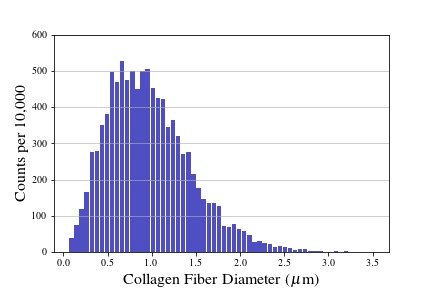
\includegraphics[width=0.475\textwidth]{figures/collagenFiberDiaHistogram.jpg}
        \label{fig:septalChordStatsC}
    }
    \hfill
    \subfigure[Histogram for elastin chord diameters.]{
        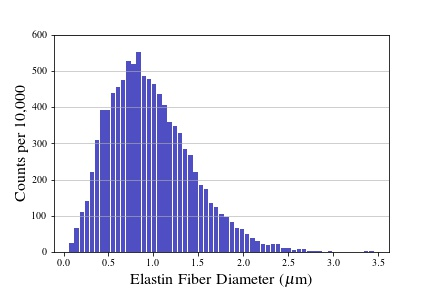
\includegraphics[width=0.475\textwidth]{figures/elastinFiberDiaHistogram.jpg}
        \label{fig:septalChordStatsE}
    }
    \caption{Typical histograms for alveolar chord diameters constructed using the statistics reported in Table~\ref{tab:alveolarProp}.  Their tails weigh heavy at the larger diameters, because their distributions are normal in the square root of their diameters.  These two histograms are virtually identical.}
    \label{fig:septalChordStats}
\end{figure}

The collagen and elastin fibers that make up a septal chord have the same length $L$, they experience the same strain $e$, and they exist at the same temperature $\theta$; therefore, we employ Eqn.~(\ref{Helmholtz1D}) as the governing constitutive equation to describe their mechanical behaviors; specifically, for the collagen fiber in an alveolar chord
\begin{subequations}
    \label{alveolarChord}
    \begin{align}
    \left\{ \begin{matrix} 
    \mathrm{d} \eta^c \\ \mathrm{d} s^c
    \end{matrix} \right\} = \begin{bmatrix}
    C^c_t - ( \alpha^c_t )^2 E^c / \rho^c \theta & 
    \alpha^c_t E^c / \rho^c \theta \\
    -\alpha^c_t E^c & E^c
    \end{bmatrix} \left\{ \begin{matrix}
    \theta^{-1} \, \mathrm{d} \theta \\ L^{-1} \, \mathrm{d} L
    \end{matrix} \right\} 
    \intertext{where $E^c = E^c_t ( \theta , e , s^c )$, and for the elastin fiber in an alveolar chord}
    \left\{ \begin{matrix} 
    \mathrm{d} \eta^e \\ \mathrm{d} s^e
    \end{matrix} \right\} = \begin{bmatrix}
    C^e_t - ( \alpha^e_t )^2 E^e / \rho^e \theta & 
    \alpha^e_t E^e / \rho^e \theta \\
    -\alpha^e_t E^e & E^e
    \end{bmatrix} \left\{ \begin{matrix}
    \theta^{-1} \, \mathrm{d} \theta \\ L^{-1} \, \mathrm{d} L
    \end{matrix} \right\}
    \end{align}
\end{subequations}
where $E^e = E^e_t ( \theta , e , s^e )$, and where $\eta^c$ and $\eta^e$ are the entropy densities (erg/g.K) for collagen and elastin; $s^c \defeq \lambda F^c / A^c_0$ and $s^e \defeq \lambda F^e / A_0^e$ are the chordal stresses (barye = $\text{dyne/cm}^2$) carried by the collagen and elastin fibers, wherein $\lambda = L/L_0$ is the fiber stretch, $A^c_0$ and $A^e_0$ are their traction-free cross-sectional areas ($\text{cm}^2$), and $F^c$ and $F^e$ are the forces (dyne) they transmit.  Parameters $C^c_t$ and $C^e_t$ are their specific heats at constant pressure (erg/g.K), $\alpha^c_t$ and $\alpha^e_t$ are their lineal thermal strain coefficients, $E^e$ and $E^e$ are their elastic moduli ($\text{dyne/cm}^2$ = $\text{erg/cm}^3$), and $\rho^c$ and $\rho^e$ are their mass densities ($\text{g/cm}^3$).  These differential equations are subject to initial conditions considered to be $s^c_0 = s^c |_{L = L_0}$, $s^e_0 = s^e |_{L = L_0}$, $\eta^c = \eta^c_0$ and $\eta^e = \eta^e_0$, where  $\eta_0^c$ and $\eta_0^e$ are their respective entropy densities at rest.  \textit{In~vivo}, $s^c_0$ and $s^e_0$ are positive valued, cf.\ Appendix~\ref{appImplicitElasticity}; whereas, \textit{ex~vivo}, $s^c_0$ and $s^e_0$ would be zero valued.  

The actual force and entropy of an individual septal chord in our alveolar model is taken to be one third of a fiber's calculated values, as determined by Eqn.~(\ref{alveolarChord}), because each alveolar chord is typically shared between three adjoining alveoli; consequently, 
\begin{equation}
    \label{septalChordCEs}
    F^f = ( A_0^c s^c + A_0^e s^e ) / 3 \lambda 
    \quad \text{and} \quad
    S^f = ( \rho^c V_0^c \eta^c + \rho^e V_0^e \eta^e ) / 3 
\end{equation}  
where $F^f$ (dyne) is a third of the fiber's force carried by a septal chord, and $S^f$ (erg/K) is a third of the fiber's entropy.

Collagen is a fiber comprised of numerous, long, slender, wavy filaments whose waviness, known as crimp, straightens under sufficient deformation \cite{Kastelicetal'78,FreedDoehring05}.  Elastin is a linked fiber network, much like an elastomer, whose filaments between crosslinks rotate to align with an axis of loading under sufficient deformation \cite{AaronGosline81,Urry89}.  Consequently, collagen and elastin both recruit constituent filaments with increasing deformation into an overall, load-bearing, fiber response.  The internal energies of collagen and elastin may therefore be thought of as being comprised of a molecular configuration energy and a mechanical strain energy.  As such, both collagen and elastin are modeled as Freed-Rajagopal biologic fibers, which are described in terms of two such internal energies.  Their model is derived from the theory of implicit elasticity, cf.\ Appendix~\ref{appImplicitElasticity}.  According to their model, Eqn.~(\ref{RajagopaleanFiber}), tangent compliances for collagen and elastin, pertinent to the hypo-elastic constitutive formulation of Eqn.~(\ref{alveolarChord}), are described by
\begin{subequations}
    \label{septalChordModuli}
    \begin{align}
	\frac{1}{E^c_t (\theta , s^c , e )} & = \frac{e_{1_{\max}}^c - e_1^c}{E_1^c e_{1_{\max}}^c + 2(s^c - s^c_0)} + \frac{1}{E_2^c} \\
    \frac{1}{E^e_t (\theta , s^e , e )} & = \frac{e_t^e - e_1^e}{E_1^e e_t^e + 2(s^e - s^e_0)} + \frac{1}{E_2^e}  
    \intertext{whose internal strains are established from}
    e_1^c & = e - \alpha^c_t \ln \left( \frac{\theta}{\theta_0} \right) - \frac{s^c - s^c_0}{E_2^c} \\
    e_1^e & = e - \alpha^e_t \ln \left( \frac{\theta}{\theta_0} \right) - \frac{s^e - s^e_0}{E_2^e}
    \end{align}
\end{subequations}
with $\theta_0$ being body temperature, i.e., 310~K.  Material constants $E_1^c$ and $E_2^c$ are the two asymptotic moduli for collagen that bound its response, i.e., $E_1^c \leq E^c_t \leq E^c_2$, while $E_1^e$ and $E_2^e$ are the two asymptotic moduli for elastin that bound its response, viz., $E^e_1 \leq E^e_t \leq E^e_2$, both having units of stress (barye = dyne/$\text{cm}^2$), with $e_{1_{\max}}^c$ and $e_{2_{\max}}^e$ being their respective transition strains (see their derivation in Appendix~\ref{appImplicitElasticity}), i.e., they are the limiting\slash maximum states of internal conformation strain.  Collagen fibers are considered to fracture whenever the strain of stretching molecular bonds exceeds $e^c_f \defeq s_f^c / E_2^c$, where $s_f^c$ is the fracture stress.  In contrast, elastin fibers are assumed to remain intact.  (Elastin ruptures at strains in excess of 250\%, which vastly exceeds the strain range that alveoli are exposed to.)

Moduli $E^c_t = E^c_1 E^c_2 / ( E^c_1 + E^c_2 )$ and $E^e_t = E^e_1 E^e_2 / ( E^e_1 + E^e_2 )$ are considered to apply for stresses less than their respective reference stress, viz., for $s^c < s^c_0$ or $s^e < s^e_0$, to which we assign values of $s^c_0 = \tfrac{1}{2} E^c_1 e^c_{1_{\max}}$ and $s^e_0 = \tfrac{1}{2} E^e_1 e^e_{1_{\max}}$.  At these reference stresses, $L$ is set to $L_0$ and therefore strain $e = 0$.  This is done to help ensure a stable numerical implementation, as long slender rods readily buckle under compressive loads---a phenomenon not modeled here.  Prestressing fibers is also nature's way of ensuring their structural integrity.

\begin{table}
    \centering
    \begin{tabular}{|l|l|l|}
        \hline
        \multicolumn{3}{|c|}{Collagen$\vphantom{|^{|^|}}$} \\ \hline
        $\rho^c$ \hfill [$\textrm{g/cm}^{3^{\phantom{|}}}$] & $1.34$ & 
        Fels \cite{Fels64} \\
        $\eta_0^c$ \hfill [erg/g.K] & $3.7 \times 10^7$ &  \\
        $C^c_p$ \hfill [erg/g.K] & $1.7 \times 10^7$ & 
        Kanagy \cite{Kanagy55} \\
        $\alpha^c_s = \alpha^c_t$ & $0.056$ & 
        Weir \cite{Weir48}  \\
        $e^c_{1_{\max}}$ & $0.09 \pm 0.018$ & estimated from TLC $\approx$ 30\% \\
        $e^c_f$ & $0.25 \pm 0.025$ & \\
        $E_1^c$ \hfill [barye] & $5.0 \pm 1.0 \times 10^5$ &  \\
        $E_2^c$ \hfill [barye] & $5.0 \pm 0.5 \times 10^7$ &  \\ 
        $s^e_0$ \hfill [barye] & $E^c_1 e^c_{1_{\max}} / 2$ & assumption \\ \hline
        \multicolumn{3}{|c|}{Elastin$\vphantom{|^{|^|}}$} \\ \hline 
        Parameter & Value & Reference \\ \hline
        $\rho^e$ \hfill [$\textrm{g/cm}^{3^{\phantom{|}}}$] & $1.31$ & 
        Lillie \& Gosline \cite{LillieGosline02a} \\
        $\eta_0^e$ \hfill [erg/g.K] & $3.4 \times 10^7$ & 
        Shadwick \& Gosline \cite{ShadwickGosline85} \\
        $C^e_p$ \hfill [$\textrm{erg/g.K}$] & $4.2 \times 10^7$  & 
        Kakivaya \& Hoeve \cite{KakivayaHoeve75} \\
        $\alpha^e_s = \alpha^e_t$ & $0.1$ & 
        Lillie \& Gosline \cite{LillieGosline02a} \\ 
        $e^e_{1_{\max}}$ & $0.4 \pm 0.08$ & Shadwick \& Gosline \cite{ShadwickGosline85} \\
        $E^e_1$ \hfill [barye] & $2.3 \pm 0.3 \times 10^6$ & Urry \cite[Fig.~18]{Urry89} \\ 
        $E^e_2$ \hfill [barye] & $1.0 \pm 0.1 \times 10^7$ & 
        Lillie \& Gosline \cite[Fig.~5]{LillieGosline07} \\
        $s^e_0$ \hfill [barye] & $E^e_1 e^e_{1_{\max}} / 2$ & assumption \\
        \hline
    \end{tabular}
    \caption{Physical properties for hydrated collagen and elastin fibers.  Collagen denatures at around $60^\circ$C \cite{HoermannSchlebusch71}, i.e., above this temperature collagen will shrink rapidly---an effect not modeled here.}
    \label{tableCollagenElastin}
\end{table}

Material properties needed to model septal chords are listed in Tables~\ref{tab:alveolarProp} \& \ref{tableCollagenElastin}.  From Eqn.~(\ref{thermodynamicConstraints}), these elastic moduli are bound from above by Eqn.~(\ref{thermodynamicConstraints}) implying that $E^c_{\max} = 2.25 \times 10^{12}$~barye ($\text{dyne/cm}^2$) and $E^e_{\max} = 1.7 \times 10^{12}$~barye.  We therefore observe that $E^c_2$ and $E^e_2$ are about $10^5$ times smaller than $E^c_{\max}$ and $E^e_{\max}$, which seems reasonable for \textit{in~vivo\/} fibers.  This theoretical upper bound for a collagen molecule is about 100 times greater than what have been measured by testing collagen fibrils under ideal laboratory conditions \cite{Svenssonetal10}.  Like results have been found for metals.

\subsection{Modeling Alveolar Septa Subjected to Shock Waves}
\label{secConjugatePairs}

The thermo\-elastic response of a planar membrane used to model alveolar septa, as described in Eqn.~(\ref{HelmholtzMembraneODEs}), is governed by the following pair of differential equations.  The first set of ODEs establishes the uniform response of a membrane, as described in Eqn.~(\ref{HelmholtzMembraneODEsUniform}), viz.,
\begin{displaymath}
    \left\{ \begin{matrix}
    \mathrm{d} \eta \\ \mathrm{d} s^{\pi}
    \end{matrix} \right\} = \begin{bmatrix}
    C_t - 4 \alpha^2_t M / \rho \theta & 
    4 \alpha_t M / \rho \theta \\
    -4 \alpha_t M & 4 M
    \end{bmatrix} \left\{ \begin{matrix}
    \theta^{-1} \, \mathrm{d} \theta \\ \mathrm{d} \xi
    \end{matrix} \right\} , \quad
    M = M_t ( \theta , s^{\pi} , \xi )
\end{displaymath}
where $s^{\pi} \defeq \pi / h$ has units of stress (dyne/$\text{cm}^2$) with $h$ denoting height or thickness of the spetal membrane.  Assuming the volume of a septal membrane remains constant, thickness would obey $h = h_0 \exp ( -2 \xi )$ with $h_0$ being its reference thickness.  Tangent modulus $M$ is an areal equivalent of the bulk modulus.  The second set of ODEs establishes the non-uniform response of a membrane, as described in Eqn.~(\ref{HelmholtzMembraneODEsNonUniform}), such that upon assuming incompressibility per Eqn.~(\ref{HelmholtzMembraneODEsNonUniformCV}), results in
\begin{displaymath}
    \left\{ \begin{matrix}
    \mathrm{d} s^{\sigma} \\ \mathrm{d} s^{\tau}
    \end{matrix} \right\} = \begin{bmatrix}
    4M/3 & 0 \\
    0 & G
    \end{bmatrix} \left\{ \begin{matrix}
    \mathrm{d} \varepsilon \\ \mathrm{d} \gamma
    \end{matrix} \right\} , \quad
        G = G_t ( s^{\tau} , \gamma )
\end{displaymath}
where $s^{\sigma} \defeq \sigma / h$ and $s^{\tau} \defeq \tau / h$ also have units of stress (dyne/$\text{cm}^2$), with $G$ being the tangent modulus for in-plane (simple) shear. 

From a mechanics perspective, we know a great deal more about alveolar chords than we know about alveolar septa.  More judgment will therefore be required in our construction and parameterization of a material model for alveolar membranes.  

A typical alveolar septum is 4-5 $\mu$m thick \cite{Sukietal11}.  They are comprised of an outside layer of epithelial cells that encase capillaries built from endothelial cells along with a basement membrane that is composed of unorganized collagen and elastin filaments, plus proteoglycans and other extracellular proteins.  This basement membrane, roughly at mid-plane in an alveolar septum, has a width of about $0.5 \, \mu$m \cite{RoanWaters11}.  Inertial forces generated by these membranes are to be based upon a membrane thickness of $\sim\!\!5$~$\mu$m with an approximate density of water, while the structural forces that they carry are to be based upon a basement membrane thickness of $\sim\!\! 0.5$~$\mu$m.  

It is not known how much of the mechanical load is actually carried by the cells in an alveolar septum vs.\ the extracellular basement membrane they encase, but it is generally thought that this basement membrane carries the majority of the load \cite{Sukietal11}.  Therefore, by diminishing the moduli that are appropriate for describing a basement membrane with thickness $\sim\!\! 0.5$~$\mu$m by a factor of 10, one gets an estimate for the effective septal moduli---an estimate applicable when modeling a whole septal membrane with thickness $\sim\!\! 5$~$\mu$m.  We employ the model parameters specified in Table~\ref{tableVisceralPleura}, which are based upon this assumption.

\begin{table}
    \centering
    \begin{tabular}{|l|l|}
        \hline
        Property & Value \\ \hline
        $\rho$ \hfill [$\textrm{g/cm}^{3^{\phantom{|}}}$] & $1.1$ \\
        $\eta_0$ \hfill [erg/g.K] & $5.0 \times 10^6$ \\
        $C_p$ \hfill [erg/g.K] & $2.1 \times 10^7$ \\
        $\alpha_t$ & $0.037$ \\ \hline
        $\xi_{1_{\max}}$ & $0.24 \pm 0.24$ \\
        $\xi_f$ & $0.2$ \\
        $M_1$ \hfill [barye] & $1.0 \pm 0.1 \times 10^4$ \\
        $M_2$ \hfill [barye] & $3.0 \pm 0.1 \times 10^6$ \\
        $s^{\pi}_0$ \hfill [barye] & $M_1 \xi_{1_{\max}} / 2$ \\ \hline
        $\gamma_{1_{\max}}$ & $3 \xi_{1_{\max}} / 2$ \\
        $G_1$ \hfill [barye] & $M_1 / 25$ \\
        $G_2$ \hfill [barye] & $M_2 / 25$ \\ \hline
    \end{tabular}
    \caption{The elastic properties reported here are for visceral pleura taken from Freed \textit{et~al}.\ \cite{Freedetal17} and parenchyma taken from Saraf \text{et~al}., \cite{Sarafetal07} divided by 10 to adjust for septal thickness vs.\ basement membrane thickness.  The thermo\-physical properties lie between that of water and collagen, weighted towards that of water, and evaluated at body temperature.}
    \label{tableVisceralPleura}
\end{table}

Collagen and elastin appear as thin filaments randomly oriented and somewhat uniformly dispersed throughout a basement membrane, unlike the strongly aligned fibers that appear in septal chords.  Furthermore, there are large numbers of proteins dispersed throughout these septa.  Consequently, for our purposes, we model this collective ensemble of tissue and structure types as a homo\-geneous isotropic membrane modeled after the Freed-Rajagopal biologic fiber \cite{FreedRajagopal16} that we have extended to membranes in App.~\ref{appImplicitElasticity}, specifically
\begin{subequations}
    \label{septalCompliances}
    \begin{align}
    \frac{1}{M_t(\theta, \xi, s^{\pi})} & = 
    \frac{\xi_{1_{\max}} - \xi_1}
    {M_1 \xi_{1_{\max}} + \tfrac{1}{2}(s^{\pi} - s^{\pi}_0)} + \frac{1}{M_2} 
    & \xi_1 & = \xi - \alpha_t \ln 
    \left( \frac{\theta}{\theta_0} \right) - \frac{s^{\pi} - s^{\pi}_0}{4M_2}
    \label{septalDilationCompliance} \\
    \intertext{and}
    \frac{1}{G_t(\gamma , s^{\tau})} & = \frac{ \mathrm{sgn} (\gamma_1) \, \gamma_{1_{\max}} - \gamma_1}{G_1 \, \mathrm{sgn} (\gamma_1) \, \gamma_{1_{\max}} + 2 s^{\tau}} + \frac{1}{G_2} & 
    \gamma_1 & = \gamma - \frac{s^{\tau}}{G_2}
    \label{septalShearCompliance}
    \end{align}
\end{subequations}
where compliant, initial, tangent moduli $M_1$ and $G_1$ and stiff, terminal, tangent moduli $M_2$ and $G_2$ bound their respective responses so that $M_1 \leq M_t \leq M_2$ and $G_1 \leq G_t \leq G_2$, with a gradual transition between their asymp\-totic bounds occurring around strains of $\xi_{1_{\max}}$ and $\gamma_{1_{\max}}$, with membrane failure or rupture being considered to only occur in the dilation mode whenever $\xi > \xi_f$.

Whenever $s^{\pi} < s^{\pi}_0$, modulus $M_t$ is assigned a value of $M_t = M_1 M_2 / ( M_1 + M_2 )$ that is the tangent modulus at reference stress $s^{\pi}_0$, which we take to be $\tfrac{1}{2} M_1 \xi_{1_{\max}}$.   Negative surface tensions cause wrinkling of a membrane surface, which is not addressed here.  In contrast, the shear modulus $G_t$ maintains applicability whenever its arguments become negative valued, which is handled via the sign function introduced in Eqn.~(\ref{septalShearCompliance}).

Finite element technology is used to interpolate entropy and stress, integrated at the Gauss points, to entropy and force at the vertices of a pentagon, which are vertices of the dodecahedron, cf.\ Part~\ref{partVariational}.  The actual entropies and forces interpolated to these nodes are halved, because each septal plane belongs to two adjoining alveoli. 

\subsection{Modeling an Alveolar Volume Subjected to Shock Waves}
\label{sec:IdealGasLaw}

Alveoli are connected to bronchial trees via alveolar ducts.  Under normal conditions, air moves in and out of the alveoli via these ducts.  However, when subjected to a stress wave passing over an alveolus, there is no time for the transport of air to take place.  Hence, we can consider the air (and heat) within an alveolus to become `trapped', and the pressure to be uniform therein.  The governing thermo\-dynamic process is therefore adiabatic.  It is under this condition that we model the volumetric response of an alveolar sac.

\subsubsection{Alveoli Filled with Air}

Considering the water saturated air within an alveolus to be an ideal gas, then \cite{Davison08}
\begin{equation}
P V = n \! R \theta
\quad \text{or} \quad
\frac{P V}{\theta} = \frac{P_0 V_0}{\theta_0} = n \! R = \mathrm{constant}
\label{idealGas}
\end{equation}
where, in our case, $P_0$ is taken to be the atmospheric pressure at sea level (1~bar or $10^5$~Pa or $10^6$~barye), with $V_0$ being that alveolar volume whereat alveolar pressure and plural pressure are both atmospheric, while $\theta_0 = 37^{\circ}$C = 310~K is assigned as body temperature.  Parameter $n$ is the molar content of gas within an alveolus, and $R$ is the universal gas constant.  

The material properties associated with an ideal gas contained within an adiabatic enclosure are
\begin{subequations}
    \label{idealGasConstants}
    \begin{align}
\alpha_t & \defeq \frac{\theta}{L} \left. \frac{\partial L}{\partial \theta} \right|_P =
\frac{\theta}{3V} \left. \frac{\partial V}{\partial \theta} \right|_P = 
\frac{1}{3\theta_0} \, \frac{P_0}{P} \frac{V_0}{V} \\
\intertext{and}
K_t & \defeq -V \left. \frac{\partial P}{\partial V} \right|_{\theta} = 
P_0 \, \frac{\theta}{\theta_0} \frac{V_0}{V} 
\label{idealGasK}
\end{align}
\end{subequations}
with the other two material properties pertaining to moist air at body temperature\footnote{
    Physical properties for air were taken from the website \texttt{www.peacesoftware.de} hosted by Berndt Wischnewski.
}
being its mass density $\rho$ of $1.125 \times 10^{-3} \; \text{g/cm}^3$ and its specific heat $C_t$ of $1.007 \times 10^7$~erg/g.K at constant pressure, constrained by $K_t < K_{\max} = \rho C_t \theta / \alpha^2_t \approx \rho C_t \theta_0 / 9 = 3.9 \times 10^5$ barye.  An alveolar sac, when modeled as an adiabatic pressure vessel filled with an ideal gas, is described by
\begin{equation}
\left\{ \begin{matrix}
    \mathrm{d} \eta \\ -3 \, \mathrm{d} P
\end{matrix} \right\} = \begin{bmatrix}
    C_t - 9 \alpha^2_t K_t / \rho \theta & 
    9 \alpha_t K_t / \rho \theta \\
    -9 \alpha_t K_t & 9 K_t
\end{bmatrix} \left\{ \begin{matrix}
    \theta^{-1} \, \mathrm{d} \theta \\ \mathrm{d} \Xi
\end{matrix} \right\}
\tag{\ref{Helmholtz3D}}
\end{equation}
where the entropy within an alveolar sac is given by $S^a = \rho V \eta$ whose initial condition is $S^a_0 = \rho V_0 \eta_0$ with $\rho \eta_0$ being the entropy per unit volume of humid air at body temperature and atmospheric pressure, viz., $\rho \eta_0 = 7.770 \times 10^4 \: \text{erg/cm}^3\text{.K}$.  Equation~(\ref{Helmholtz3D}) in conjunction with the physical properties describing an ideal gas given in Eqn.~(\ref{idealGasConstants}) result in the following differential equation governing pressure
\begin{displaymath}
\frac{\mathrm{d} P}{P} = \frac{P_0}{P} \frac{V_0}{V} \frac{\theta}{\theta_0} \left( 
\frac{P_0}{P} \frac{V_0}{V} \frac{\theta}{\theta_0} \, 
\frac{\mathrm{d} \theta}{\theta} - 
\frac{\mathrm{d} V}{V} \right)
\end{displaymath}
wherein pressure, volume and temperature all appear as logarithmic rates.

Pressure $P$ is mapped to nodal forces at the vertices of a dodecahedron in our alveolar model.  This requires finite element technology, which is discussed in Part~\ref{partVariational}.

\subsubsection{Alveoli Filled with Fluid}

In lung tissues that are not healthy, fluids may fill alveolar volumes at various regions throughout a lung, e.g., as could have been caused by injury, pneumonia, etc.  In such localities the mechanical response of the local parenchyma will be vastly stiffer than that of healthy tissue, and as such, it will respond very differently to an imposed traveling shock wave.  For example, the speed of a wave moving over alveoli filled with fluid will be several orders in magnitude faster than the speed of the same wave moving over healthy alveoli filled with air.

In the presence of a passing shock wave, we suppose that an unhealthy alveolar sac, like a healthy one, can be modeled as an adiabatic enclosure, but now the fluid within such an alveolus is considered to behave, momentarily, like an elastic solid, viz., as the glassy, elastic, upper-bound response of a visco\-elastic liquid, which blood is, for example.

The thermo\-elastic response of an alveolar volume, as described in Eqn.~(\ref{HelmholtzODEs}), is governed by three sets of uncoupled differential equations.  The first set of ODEs establishes the uniform response of Eqn.~(\ref{HelmholtzODEsUniform}) described by
\begin{displaymath}
\left\{ \begin{matrix}
\mathrm{d} \eta \\ \mathrm{d} \Pi 
\end{matrix} \right\} = \begin{bmatrix}
C_t - 9 \alpha^2_t K / \rho \theta & 9 \alpha_t K / \rho \theta \\
-9 \alpha_t K & 9K
\end{bmatrix} \left\{ \begin{matrix}
\theta^{-1} \, \mathrm{d} \theta \\ \mathrm{d} \Xi 
\end{matrix} \right\} , \quad
K = K_t ( \theta , \Pi , \Xi )
\end{displaymath}
with the second set of ODEs in Eqn.~(\ref{HelmholtzODEsSqueeze}) governing the squeeze response
\begin{displaymath}
\left\{ \begin{matrix}
\mathrm{d} \sigma_1 \\ \mathrm{d} \sigma_2
\end{matrix} \right\} = \frac{3}{2} \begin{bmatrix}
2 N_1 & -N_2 \\
-N_1 & 2N_2
\end{bmatrix} \left\{ \begin{matrix}
\mathrm{d} \varepsilon_1 \\ \mathrm{d} \varepsilon_2
\end{matrix} \right\} , \quad
\begin{aligned}
N_1 & = N_t ( \sigma_1 , \varepsilon_1 ) \\
N_2 & = N_t ( \sigma_2 , \varepsilon_2 )
\end{aligned}
\end{displaymath}
while the third set of ODEs in Eqn.~(\ref{HelmholtzODEsShear}) governs the shear response
\begin{displaymath}
    \left\{ \begin{matrix}
    \mathrm{d} \tau_1 \\ \mathrm{d} \tau_2 \\ \mathrm{d} \tau_3
    \end{matrix} \right\} = \begin{bmatrix}
    G_1 & 0 & 0 \\ 0 & G_2 & 0 \\ 0 & 0 & G_3
    \end{bmatrix} \left\{ \begin{matrix}
    \mathrm{d} \gamma_1 \\ \mathrm{d} \gamma_2 \\ \mathrm{d} \gamma_3
    \end{matrix} \right\} , \quad
    \begin{aligned}
    G_1 & = G_t ( \tau_1 , \gamma_1 ) \\
    G_2 & = G_t ( \tau_2 , \gamma_2 ) \\
    G_3 & = G_t ( \tau_3 , \gamma_3 )
    \end{aligned}
\end{displaymath}
that, collectively, can be used to describe the thermo\-elastic response of a volume of material.  

How these are to be parameterized will be addressed in next year's work.


\section{Code Verification and Capabilities of the Constitutive Equations}
\label{secCE_verifyCode}

\begin{figure}
    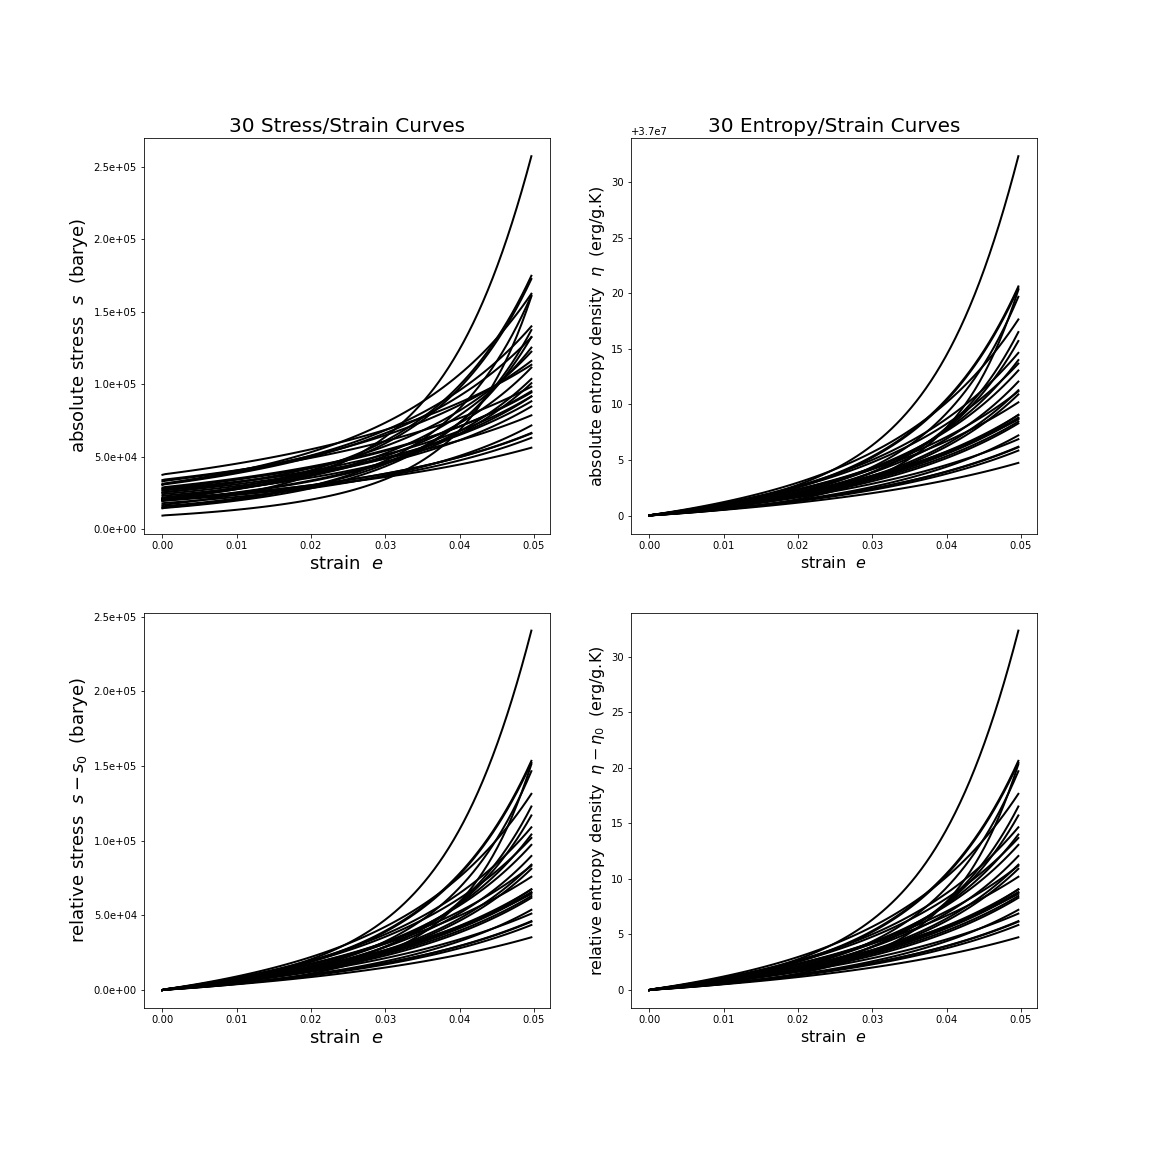
\includegraphics[width=\textwidth]{figures/bioFibers5.jpg}
    \caption{Typical stress\slash strain (left column) and entropy\slash strain (right column) response curves for collagen fibers loaded \textit{in~vivo\/} to 5\%\ strain. The top row presents their absolute responses, while the bottom row presents their relative responses.  A reference fiber length, whereat strain is arbitrarily set to zero, has been selected to associate with half the available stretch that can be attributed to molecular reconfiguration.}
    \label{figCollagenFibersInVivo}
\end{figure}

Figure \ref{figCollagenFibersInVivo} illustrates what a typical thermo-mechanical response for a collagen fiber would be expected to look like \textit{in~vivo\/} (top row) and \textit{ex~vivo\/} (bottom row) for thirty typical fibers, as predicted by the Freed-Rajagopal \cite{FreedRajagopal16} model derived in \S\ref{secBioFiber} of this appendix.  The \textit{in~vivo\/} response typifies how fibers are prestressed in the various alveolar structures of paraenchyma.  The material properties for collagen used to create this figure came from Table~\ref{tableCollagenElastin}. Stress\slash strain curves are shown in the left column, while entropy\slash strain curves are shown in the right column.  The top row provides their absolute responses, while the bottom row provides their relative responses.  \textit{In~vivo}, biologic fibers do not associate with reference states that are void of stress.  This is apparent in the upper-left graph ($s$ vs.\ $e$), whose response is normalized in the lower-left graph ($s \! - \! s_0$ vs.\ $e$), and likewise for entropy.  The graphs that follow will plot relative values.

Figure~\ref{figCollagenFibersInVivo} presents stress\slash strain and entropy\slash strain response curves out to 5\%\ strain.  Figure~\ref{figCollagenFiber} extends the deformation out to 10\%, 20\%, 30\%\ and 40\%\ strains.  In all of these figures we observe that any additional contribution to the entropy caused by deformation can be neglected (it being less than 1 part out of $10^4$).  In addition to possessing a capability of having stressed fibers in their reference state, established via $s_0 \defeq \tfrac{1}{2} E_1 e_{1_{\max}}$ and as seen in Fig.~\ref{figCollagenFibersInVivo}, our fiber model also accounts for fiber rupture, which is considered to be triggered at a maximum stress of $s_f \defeq E_2 e_f$.  Ruptures start at around 30\%\ strain for the specified material parameters.  In these figures, material properties  $E_1$, $E_2$ and $e_{1_{\max}}$ for collagen were all assigned random values according to their respective probabilistic distributions taken from Table~\ref{tableCollagenElastin}.  Employing 75 steps to integrate each response (sufficient for drawing nice curves) results in numerical errors of integration (right column in Fig.~\ref{figCollagenFiber}), specifically, in local truncation errors that were found to be on the order of the square root of machine precision, which is considered to be very good.

\begin{figure}
    \mbox{}\hspace{-1.5cm}
    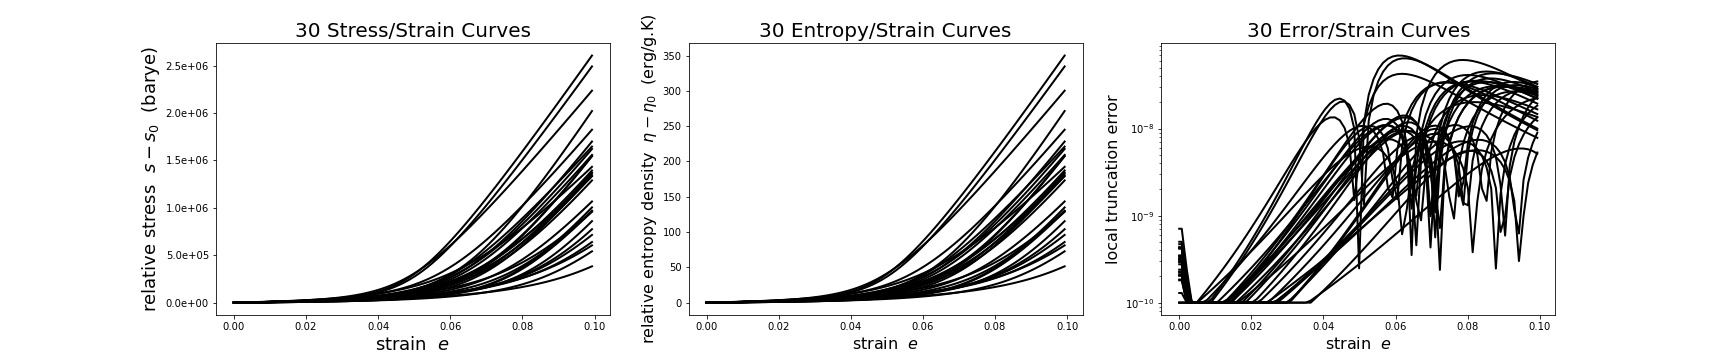
\includegraphics[width=1.2\textwidth]{figures/bioFibers10.jpg}
    \mbox{}\hspace{-1.5cm}
    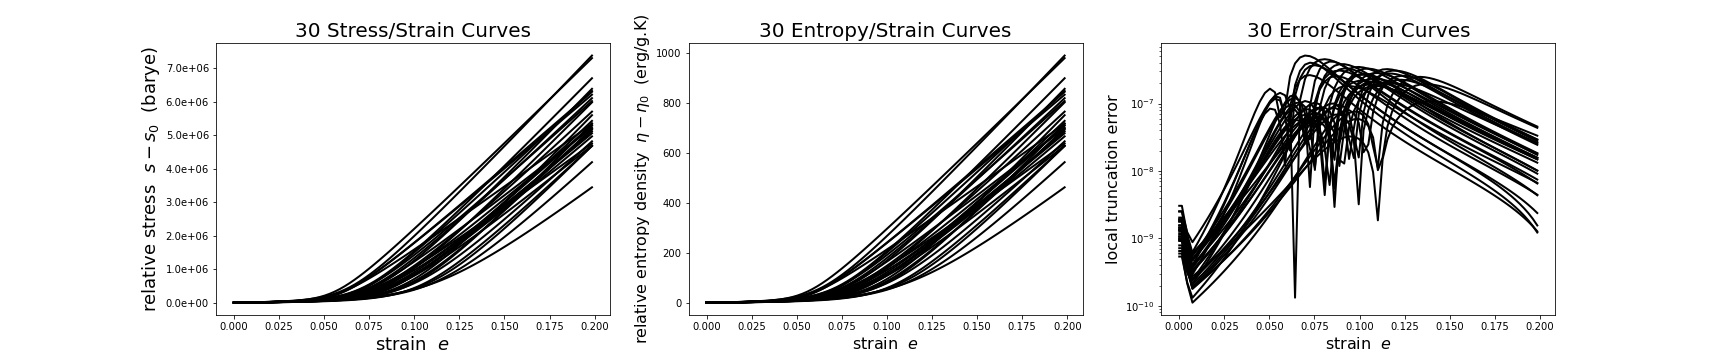
\includegraphics[width=1.2\textwidth]{figures/bioFibers20.jpg}
    \mbox{}\hspace{-1.5cm}
    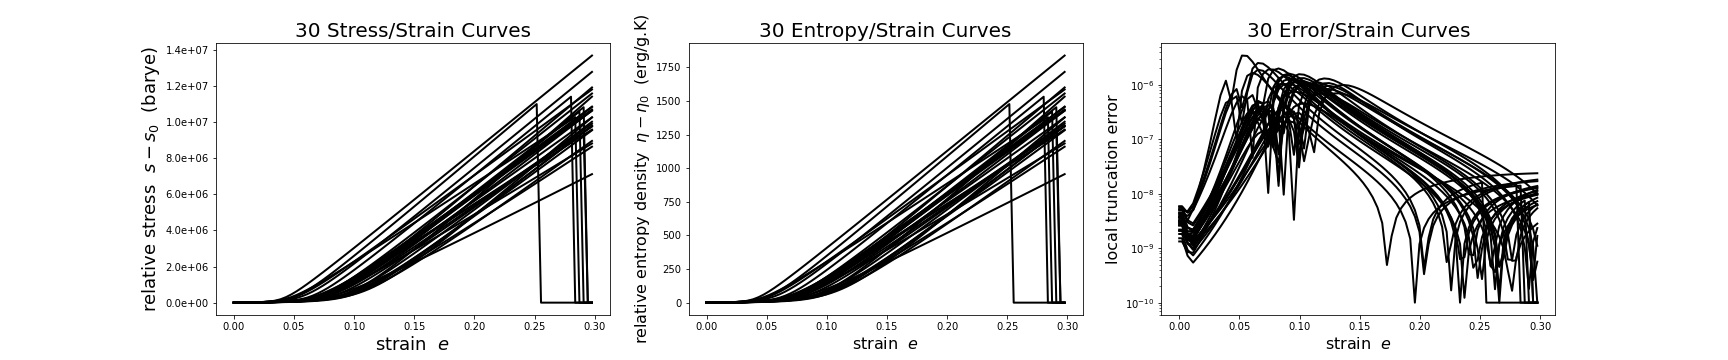
\includegraphics[width=1.2\textwidth]{figures/bioFibers30.jpg}
    \mbox{}\hspace{-1.5cm}
    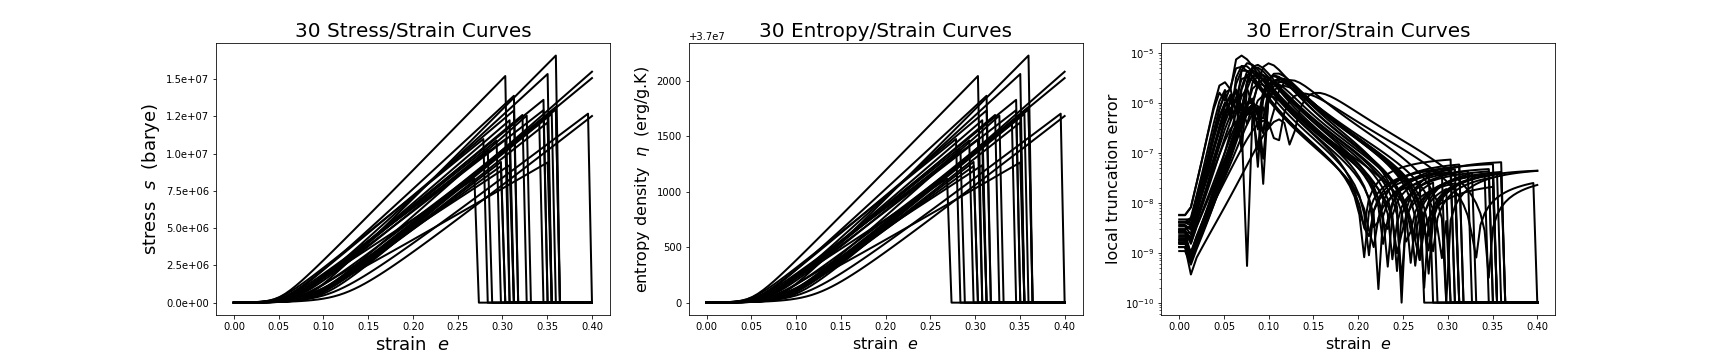
\includegraphics[width=1.2\textwidth]{figures/bioFibers40.jpg}
    \caption{Stress\slash strain (left column), entropy density\slash strain (center column), and local truncation error\slash strain (right column) curves for collagen using the material parameters listed in Table~\ref{tableCollagenElastin}, which are described in terms of probability distributions.  The top row is for strains out to 10\%, the second row is for strains out to 20\%, the third row is for strains out to 30\%, and the fourth row is for strains out to 40\%.  There were no fiber failures in those that were stretched out to 10\%\ and 20\%\ strain.  Six of the thirty fibers failed in those stretched out to 30\%\ strain, while twenty eight of the thirty fibers failed for those stretched out to 40\%\ strain.  The local truncation errors plotted here associate with the PECE integrator presented in Eqn.~(\ref{1stOrderODEs}) of Part~\ref{partNumericalMethods} using 75 steps of integration, with errors less than $10^{-10}$ set at $10^{-10}$.  The reported truncation errors never exceeded 0.001\%.}
    \label{figCollagenFiber}
\end{figure}

Like Figs.~\ref{figCollagenFibersInVivo} \&\ \ref{figCollagenFiber}, material properties $E_1$, $E_2$ and $e_{1_{\max}}$ were each assigned random values for both elastin and collagen using parameters taken from Table~\ref{tableCollagenElastin} for the purpose of constructing the 30 curves presented in each plot of Fig.~\ref{figStressStrainFibers} for septal chords.  Plus, their fiber lengths and diameters were likewise assigned random values according to their respective probabilistic distributions taken from Fig.~(\ref{septalLengthFig}), using formula (\ref{dodecahedralHeight}), and the data from Table~\ref{tab:alveolarProp}.  Figure~\ref{figStressStrainFibers} presents realistic variability with what one should expect for chordal responses in the alveoli of lung.  Both the chordal force and entropy (actual entropy, not entropy density) were calculated using the rule of mixtures based upon volume fractions of collagen vs.\ elastin.  The change in chordal entropy was so small that variability caused by variation in volume fraction dominates this response; hence, relative changes in entropy ($S \! - \! S_0$) had to be plotted to visualize the effect.  In the septal chords that failed during this analysis, it was collagen fibers that ruptured with elastin fibers continuing to carry load.  

\begin{figure}
    \mbox{}\hspace{-1.5cm}
    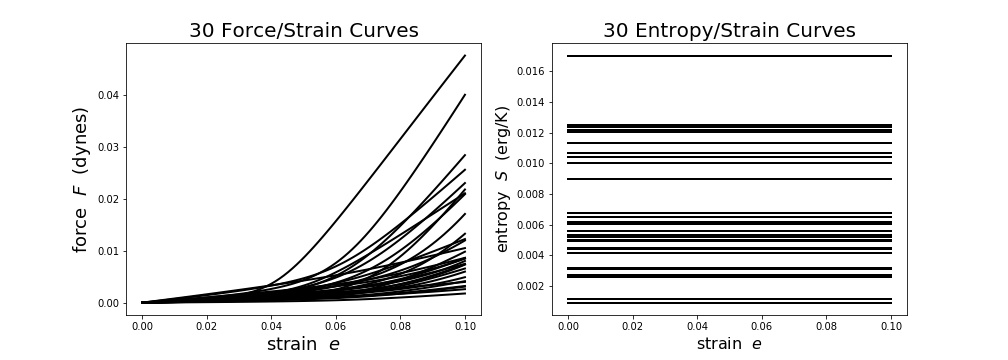
\includegraphics[width=1.2\textwidth]{figures/septalChords10.jpg}
    \mbox{}\hspace{-1.5cm}
    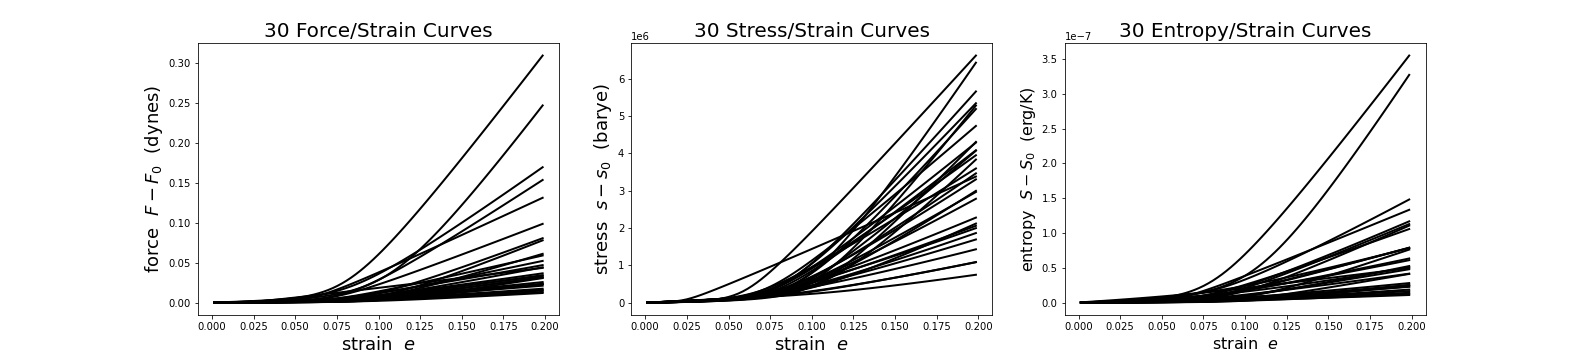
\includegraphics[width=1.2\textwidth]{figures/septalChords20.jpg}
    \mbox{}\hspace{-1.5cm}
    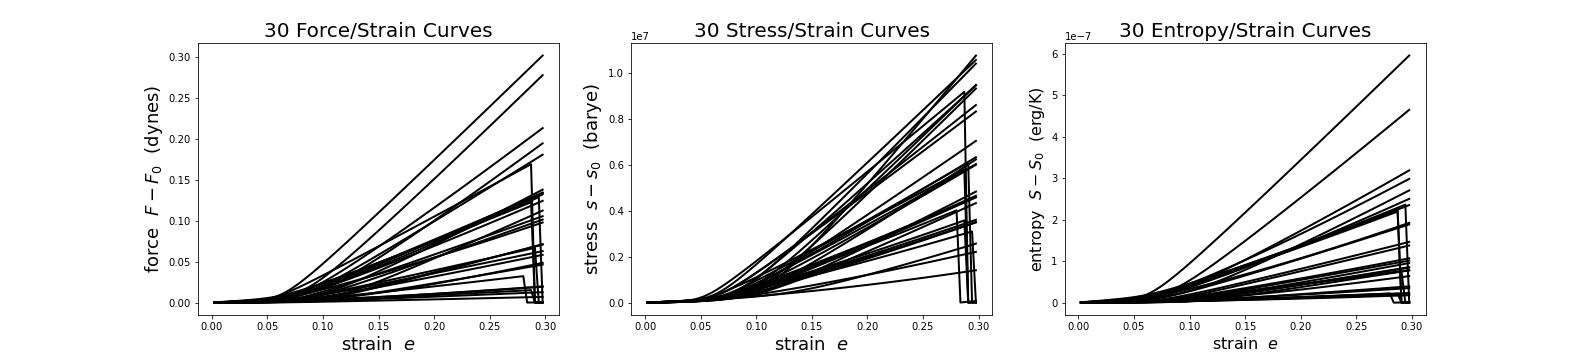
\includegraphics[width=1.2\textwidth]{figures/septalChords30.jpg}
    \mbox{}\hspace{-1.5cm}
    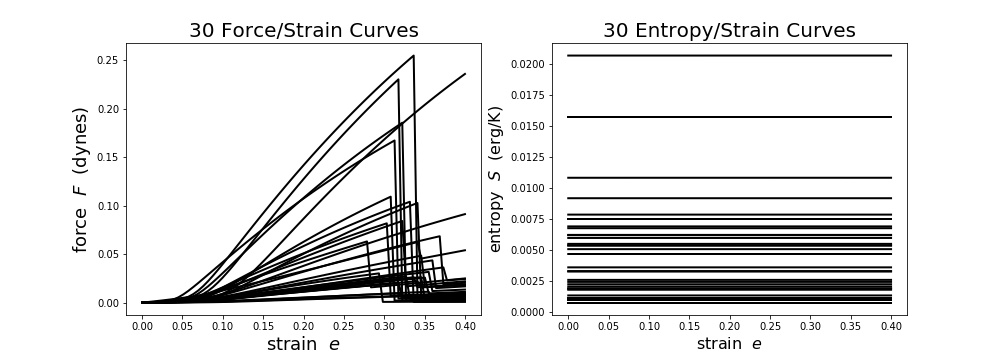
\includegraphics[width=1.2\textwidth]{figures/septalChords40.jpg}
    \caption{Relative force\slash strain (left column), relative nominal stress\slash strain (center column), and relative entropy\slash strain (right column) curves for septal chords comprised of individual collagen and elastin fibers whose material parameters are listed in Table~\ref{tableCollagenElastin}, which are described in terms of probability distributions.  The top row is for strains out to 10\%, the second row is for strains out to 20\%, the third row is for strains out to 30\%, and the fourth row is for strains out to 40\%.  There were no fiber failures in those that were stretched out to 10\%\ and 20\%\ strain.  Six of the thirty collagen fibers failed in those stretched out to 30\%\ strain with none of the elastin fibers failing, while twenty nine of the thirty collagen fibers failed for those stretched out to 40\%\ strain, again, with none of the elastin fibers failing.}
    \label{figStressStrainFibers}
\end{figure}

The three conjugate pairs that describe a membrane's response are presented as rows in Fig.~\ref{figStressStrainMembranes}---one row per experiment, with there being 30 curves per plot.  These conjugate pairs describe: uniform dilation $( s^{\pi} , \xi )$, non-uniform squeeze $( s^{\sigma} , \varepsilon )$, and non-uniform (simple) shear $( s^{\tau} , \gamma )$.  The three motions that we consider include: \newline dilation
\begin{subequations}
    \label{membraneExperiments}
    \begin{align}
    a & = \lambda & b & = \lambda & g - g_0 & = 0 
    \label{dilationExperiment}\\
    \intertext{pure shear \cite{FreedSrinivasa15}}
    a & = \frac{\sqrt{\lambda^2 + \lambda^{-2}}}{\sqrt{2}} & 
    b & = \frac{\sqrt{2}}{\sqrt{\lambda^2 + \lambda^{-2}}} & g - g_0 &  = 
    \frac{\lambda^2 - \lambda^{-2}}{\lambda^2 + \lambda^{-2}} 
    \label{pureShearExperiment} \\
    \intertext{and simple shear}
    a & = 1 & b & = 1 & g - g_0 & \neq 0
    \label{simpleShearExperiment}
    \end{align}
\end{subequations}
where $\lambda$ denotes a stretch with $\lambda_0 = 1$.  For dilation: $\xi = \ln \lambda$, $\varepsilon = 0$ \&\ $\gamma = 0$; for pure shear: $\xi = 0$, $\varepsilon = \ln \bigl( \tfrac{1}{2} ( \lambda^2 + \lambda^{-2}) \bigr)$ \&\ $\gamma = ( \lambda^2 - \lambda^{-2} ) / (\lambda^2 + \lambda^{-2})$; and for simple shear: $\xi = 0$, $\varepsilon = 0$ \&\ $\gamma = g - g_0$.
The constitutive model is that of Eqns.\ (\ref{HelmholtzMembraneODEs} \& \ref{septalCompliances}), applying material parameters (and their variability) given in Table~\ref{tableVisceralPleura}.  In the dilation experiment (top row) there is only uniform $( s^{\pi} \! , \xi)$ response.  There are no non-uniform responses, neither $( s^{\sigma} \! , \varepsilon)$ nor $( s^{\tau} \! , \gamma)$ in an uniform dilation, either theoretical or numerical.  The conjugate pairs are uncoupled here.  Likewise, in the simple shear experiment (bottom row) there is only a non-uniform $( s^{\tau} \! , \gamma)$ response.  Theoretically, there is neither uniform $( s^{\pi} \! , \xi)$ nor non-uniform $( s^{\sigma} \! , \varepsilon)$ responses in a non-uniform simple shear.  However, we observe some numerical error arising in the uniform response---on the order of 1 part in $10^{12}$ and, therefore, negligible.  The pure shear experiment (middle row) is dominated by both a squeeze $( s^{\sigma} \! , \varepsilon)$ and a shear  $( s^{\tau} \! , \gamma)$ response, with there being a small, systematic, dilational coupling through pair $( s^{\pi} \! , \xi)$ that is on the order of 1 part in $10^6$.  This is the greatest numerical error in our implementation, but still it is sufficiently small so that it can be neglected without concern.  Eight of the thirty dilation experiments presented here resulted in membrane rupture.  As currently modeled, rupture only associates with the dilational response in septal membranes.

\begin{figure}
    \mbox{} \hspace{-25mm}
    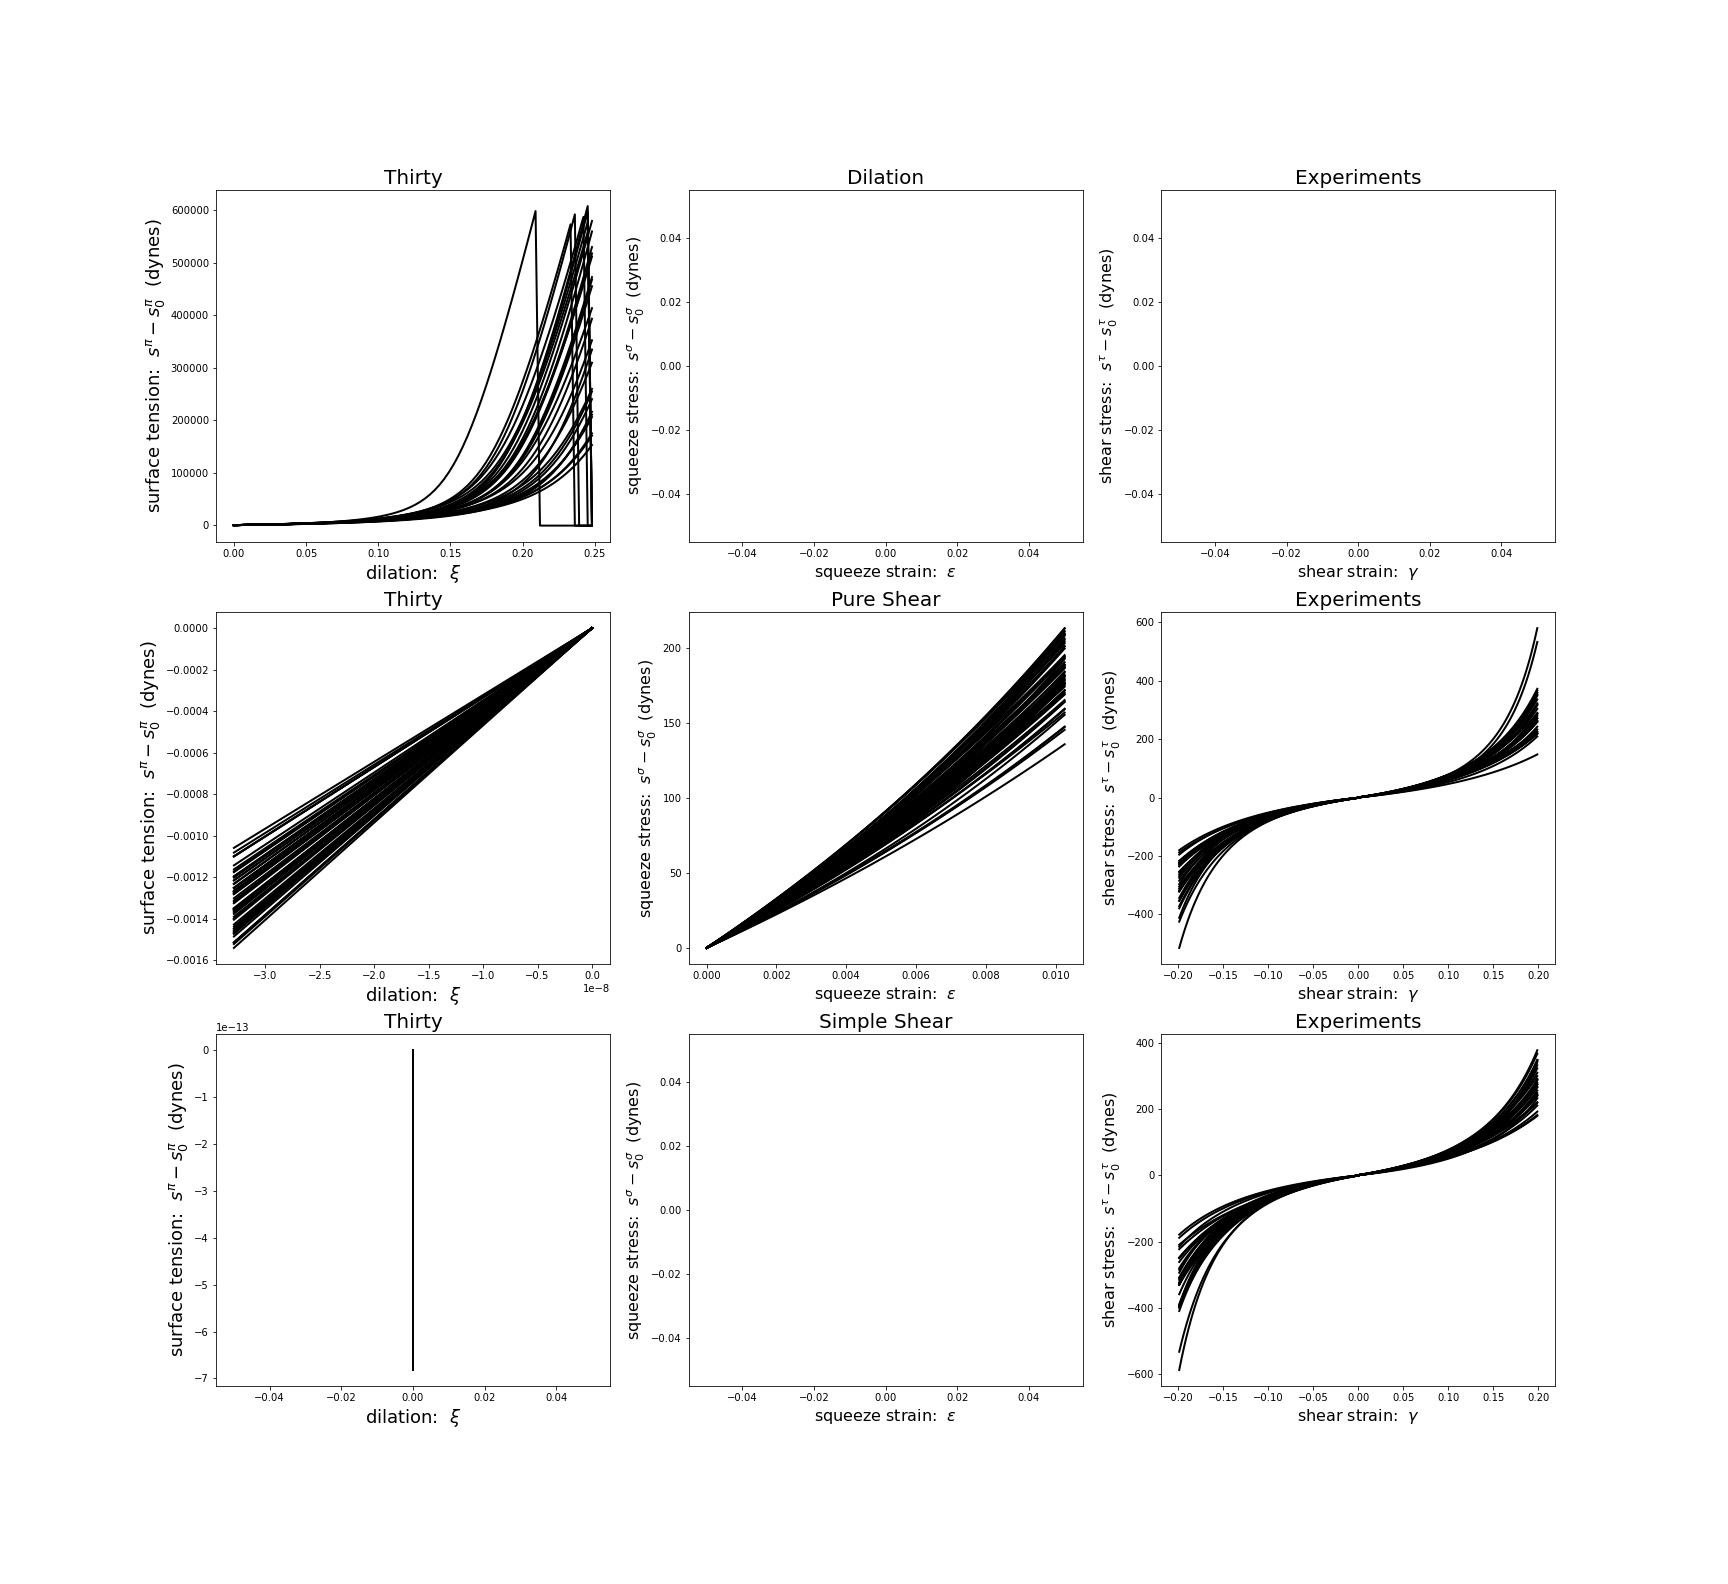
\includegraphics[width=1.3\textwidth]{figures/septalMembranes.jpg}
    \caption{Membrane response from thirty numerical experiments whose constitutive behavior is described by Eqns.~(\ref{HelmholtzMembraneODEs} \& \ref{septalCompliances}) using the parameters listed in Table~\ref{tableVisceralPleura}. The first column gives the $( s^{\pi} \! - \! s_0^{\pi} , \xi)$ conjugate pair response, the second column gives the $( s^{\sigma} \! - s_0^{\sigma} , \varepsilon)$ conjugate pair response, while the third column gives the $( s^{\tau} \! - \! s_0^{\tau} , \gamma)$ conjugate pair response.  The first row represents a dilation experiment described by Eqn.~(\ref{dilationExperiment}), the second row represents a pure shear experiment described by Eqn.~(\ref{pureShearExperiment}), while the third row represents a simple shear experiment described by Eqn.~(\ref{simpleShearExperiment}).  During these numerical experiments, eight membranes ruptured under dialation, while none ruptured during these pure and simple shear experiments.}
    \label{figStressStrainMembranes}
\end{figure}

Recently, Birzle \textit{et~al}.\ \cite{Birzleetal19} performed experiments on thin slices of rat parenchyma loaded in tension where they removed the collagen and\slash or elastin fiber content through collagenase and elastase treatment baths to study their individual behaviors and their interactions under load.

\textbf{Observation}: The change in entropy caused by deformation has been shown to be negligible when compared with the entropy present in its reference state.  As such, entropy and its conjugate, i.e., temperature, will not be modeled in our finite element representations of alveoli being exposed to traveling shock waves.
